\chapter{Solid Mechanics Model\index{SolidMechanicsModel}\label{sect:smm}}

The solid mechanics model is a specific implementation of the
\code{Model} interface dedicated to handle the equations of motion or
equations of equilibrium. The model is created for a given mesh.  It
will create its own \code{FEEngine} object to compute the interpolation,
gradient, integration and assembly operations.  A
\code{SolidMechanicsModel} object can simply be created like this:
\begin{cpp}
  SolidMechanicsModel model(mesh);
\end{cpp}
where \code{mesh} is the mesh for which the equations are to be
solved. A second parameter called \code{spatial\_dimension} can be
added after \code{mesh} if the spatial dimension of the problem is
different than that of the mesh.

This model contains at least the following six \code{Arrays}:
\begin{description}
\item[blocked\_dofs] contains a Boolean value for each degree of
  freedom specifying whether that degree is blocked or not. A
  Dirichlet boundary condition can be prescribed by setting the
  \textbf{blocked\_dofs} value of a degree of freedom to \code{true}.
  A Neumann boundary condition can be applied by setting the
  \textbf{blocked\_dofs} value of a degree of freedom to \code{false}.
  The \textbf{displacement}, \textbf{velocity} and
  \textbf{acceleration} are computed for all degrees of freedom for
  which the \textbf{blocked\_dofs} value is set to \code{false}. For
  the remaining degrees of freedom, the imposed values (zero by
  default after initialization) are kept.
\item[displacement] contains the displacements of all degrees of
  freedom. It can be either a computed displacement for free degrees
  of freedom or an imposed displacement in case of blocked ones
  ($\vec{u}$ in the following).
\item[velocity] contains the velocities of all degrees of freedom.  As
  \textbf{displacement}, it contains computed or imposed velocities
  depending on the nature of the degrees of freedom ($\dot{\vec{u}}$
  in the following).
\item[acceleration] contains the accelerations of all degrees of
  freedom. As \textbf{displacement}, it contains computed or imposed
  accelerations depending on the nature of the degrees of freedom
  ($\ddot{\vec{u}}$ in the following).
\item[external\_force] contains the external forces applied on the nodes
  ($\vec{f}_{\st{ext}}$ in the following).
\item[internal\_force] contains the internal forces on the nodes
  ($\vec{f}_{\st{int}}$ in the following).
\end{description}

Some examples to help to understand how to use this model will be
presented in the next sections.

\section{Model Setup}


\subsection{Setting Initial Conditions \label{sect:smm:initial_condition}}

For a unique solution of the equations of motion, initial
displacements and velocities for all degrees of freedom must be
specified:
\begin{eqnarray}
  \vec{u}(t=0) = \vec{u}_0\\
  \dot{\vec u}(t=0) =\vec{v}_0
\end{eqnarray} The solid mechanics model can be initialized as
follows:
\begin{cpp}
  model.initFull()
\end{cpp}
This function initializes the internal arrays and sets them to
zero. Initial displacements and velocities that are not equal to zero
can be prescribed by running a loop over the total number of
nodes. Here, the initial displacement in $x$-direction and the
initial velocity in $y$-direction for all nodes is set to $0.1$ and $1$,
respectively.
\begin{cpp}
auto & disp = model.getDisplacement();
auto & velo = model.getVelocity();

for (UInt node = 0; node < mesh.getNbNodes(); ++node) {
  disp(node, 0) = 0.1;
  velo(node, 1) = 1.;
}
\end{cpp}

\subsection{Setting Boundary Conditions\label{sect:smm:boundary}}
This section explains how to impose Dirichlet or Neumann boundary
conditions. A Dirichlet boundary condition specifies the values that
the displacement needs to take for every point $x$ at the boundary
($\Gamma_u$) of the problem domain (Fig.~\ref{fig:smm:boundaries}):
\begin{equation}
  \vec{u} = \bar{\vec u} \quad \forall \vec{x}\in
  \Gamma_{u}
\end{equation}
A Neumann boundary condition imposes the value of the gradient of the
solution at the boundary $\Gamma_t$ of the problem domain
(Fig.~\ref{fig:smm:boundaries}):
\begin{equation}
  \vec{t} = \mat{\sigma} \vec{n} = \bar{\vec t} \quad
  \forall \vec{x}\in \Gamma_{t}
\end{equation}

\begin{figure} \centering
\def\svgwidth{0.5\columnwidth}
  \input{figures/problemDomain.pdf_tex}
  \caption{Problem domain $\Omega$ with boundary in three
    dimensions. The Dirchelet and the Neumann regions of the boundary
    are denoted with $\Gamma_u$ and $\Gamma_t$,
    respecitvely.\label{fig:smm:boundaries}}
  \label{fig:problemDomain}
\end{figure}

Different ways of imposing these boundary conditions exist. A basic
way is to loop over nodes or elements at the boundary and apply local
values. A more advanced method consists of using the notion of the
boundary of the mesh. In the following both ways are presented.

Starting with the basic approach, as mentioned, the Dirichlet boundary
conditions can be applied by looping over the nodes and assigning the
required values. Figure~\ref{fig:smm:dirichlet_bc} shows a beam with a
fixed support on the left side. On the right end of the beam, a load
is applied. At the fixed support, the displacement has a given
value. For this example, the displacements in both the $x$ and the
$y$-direction are set to zero. Implementing this displacement boundary
condition is similar to the implementation of initial displacement
conditions described above. However, in order to impose a displacement
boundary condition for all time steps, the corresponding nodes need to
be marked as boundary nodes using the function \code{blocked}. While, 
in order to impose a load on the right side, the nodes are not marked.
The detail codes are shown as follows:

\begin{cpp}
auto & blocked = model.getBlockedDOFs();
const auto & pos = mesh.getNodes();

UInt nb_nodes = mesh.getNbNodes();

for (UInt node = 0; node < nb_nodes; ++node) {
  if(Math::are_float_equal(pos(node, _x), 0)) {
    blocked(node, _x) = true; // block dof in x-direction
    blocked(node, _y) = true; // block dof in y-direction
    disp(node, _x) = 0.; // fixed displacement in x-direction
    disp(node, _y) = 0.; // fixed displacement in y-direction
  } else if (Math::are_float_equal(pos(node, _y), 0)) {
    blocked(node, _x) = false; // unblock dof in x-direction
    forces(node, _x) = 10.;    // force in x-direction
  }
}
\end{cpp}

\begin{figure}[!htb]
  \centering
  \includegraphics[scale=0.4]{figures/dirichlet}
  \caption{Beam with fixed support and load.\label{fig:smm:dirichlet_bc}}
\end{figure}


For the more advanced approach, one needs the notion of a boundary in
the mesh. Therefore, the boundary should be created before boundary
condition functors can be applied. Generally the boundary can be
specified from the mesh file or the geometry.  For the first case, the
function \code{createGroupsFromMeshData} is called.  This function
can read any types of mesh data which are provided in the mesh
file. If the mesh file is created with Gmsh, the function takes one
input strings which is either \code{tag\_0}, \code{tag\_1} or
\code{physical\_names}. The first two tags are assigned by Gmsh to
each element which shows the physical group that they belong to. In
Gmsh, it is also possible to consider strings for different groups of
elements. These elements can be separated by giving a string
\code{physical\_names} to the function
\code{createGroupsFromMeshData}:
\begin{cpp}
mesh.createGroupsFromMeshData<std::string>("physical_names").
\end{cpp}
Boundary conditions support can also be
created from the geometry by calling
\code{createBoundaryGroupFromGeometry}. This function gathers all the
elements on the boundary of the geometry.

To apply the required boundary conditions, the function \code{applyBC}
needs to be called on a \code{SolidMechanicsModel}. This function
gets a Dirichlet or Neumann functor and a string which specifies the
desired boundary on which the boundary conditions is to be
applied. The functors specify the type of conditions to apply. Three
built-in functors for Dirichlet exist: \code{FlagOnly, FixedValue,}
and \code{IncrementValue}. The functor \code{FlagOnly} is used if a
point is fixed in a given direction. Therefore, the input parameter to
this functor is only the fixed direction. The \code{FixedValue}
functor is used when a displacement value is applied in a fixed
direction. The \code{IncrementValue} applies an increment to the
displacement in a given direction. The following code shows the
utilization of three functors for the top, bottom and side surface of
the mesh which were already defined in the Gmsh file:

\begin{cpp}
model.applyBC(BC::Dirichlet::FixedValue(13.0, _y), "Top");

model.applyBC(BC::Dirichlet::FlagOnly(_x), "Bottom");

model.applyBC(BC::Dirichlet::IncrementValue(13.0, _x), "Side");
\end{cpp}

To apply a Neumann boundary condition, the applied traction or stress
should be specified before. In case of specifying the traction on the
surface, the functor \code{FromTraction} of Neumann boundary
conditions is called. Otherwise, the functor \code{FromStress} should
be called which gets the stress tensor as an input parameter.

\begin{cpp}
Vector<Real> surface_traction = {0., 0., 1.};
auto surface_stress(3, 3) = Matrix<Real>::eye(3);

model.applyBC(BC::Neumann::FromTraction(surface_traction), "Bottom");

model.applyBC(BC::Neumann::FromStress(surface_stress), "Top");
\end{cpp}

If the boundary conditions need to be removed during the simulation, a
functor is called from the Neumann boundary condition to free those
boundary conditions from the desired boundary.

\begin{cpp}
 model.applyBC(BC::Neumann::FreeBoundary(), "Side");
\end{cpp}

User specified functors can also be implemented.  A full example for
setting both initial and boundary conditions can be found in
\shellcode{\examplesdir/boundary\_conditions.cc}.  The problem solved
in this example is shown in Fig.~\ref{fig:smm:bc_and_ic}. It consists
of a plate that is fixed with movable supports on the left and bottom
side. On the right side, a traction, which increases linearly with the
number of time steps, is applied. The initial displacement and
velocity in $x$-direction at all free nodes is zero and two
respectively.
\begin{figure}[!htb]
  \centering
  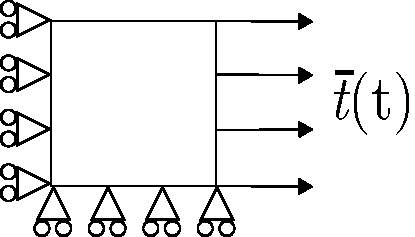
\includegraphics[scale=0.8]{figures/bc_and_ic_example}
  \caption{Plate on movable supports.\label{fig:smm:bc_and_ic}}
\end{figure}

As it is mentioned in Section \ref{sect:common:groups}, node and
element groups can be used to assign the boundary conditions. A
generic example is given below with a Dirichlet boundary condition.

\begin{cpp}
  // create a node group
  NodeGroup & node_group = mesh.createNodeGroup("nodes_fix");

  /*
  fill the node group with the nodes you want
  */

  // create an element group using the existing node group
  mesh.createElementGroupFromNodeGroup("el_fix", "nodes_fix", spatial_dimension-1);

  // boundary condition can be applied using the element group name
  model.applyBC(BC::Dirichlet::FixedValue(0.0, _x), "el_fix");
\end{cpp}

\subsection{Material Selector\label{sect:smm:materialselector}}

If the user wants to assign different materials to different
finite elements groups in \akantu, a material selector has to be
used. By default, \akantu assigns the first valid material in the
material file to all elements present in the model (regular continuum
materials are assigned to the regular elements and cohesive materials
are assigned to cohesive elements or element facets).

To assign different materials to specific elements, mesh data
information such as tag information or specified physical names can be
used. \code{MeshDataMaterialSelector} class uses this information to
assign different materials. With the proper physical name or tag name
and index, different materials can be assigned as demonstrated in the
examples below.

\begin{cpp}
  auto mat_selector = std::make_shared<MeshDataMaterialSelector<std::string>>("physical_names", model);
  model.setMaterialSelector(mat_selector);
\end{cpp}

In this example the physical names specified in a GMSH geometry file will by
used to match the material names in the input file.

Another example would be to use the first (\code{tag\_0}) or the second
(\code{tag\_1}) tag associated to each elements in the mesh:

\begin{cpp}
  auto mat_selector = std::make_shared<MeshDataMaterialSelector<UInt>>(
      "tag_1", model, first_index);
  model.setMaterialSelector(*mat_selector);
\end{cpp}

where \code{first\_index} (default is 1) is the value of \code{tag\_1} that will
be associated to the first material in the material input file. The following
values of the tag will be associated with the following materials.

There are four different material selectors pre-defined in
\akantu. \code{MaterialSelector} and \code{DefaultMaterialSelector} is
used to assign a material to regular elements by default. For the
regular elements, as in the example above,
\code{MeshDataMaterialSelector} can be used to assign different
materials to different elements. 

Apart from the \akantu's default material selectors, users can always
develop their own classes in the main code to tackle various
multi-material assignment situations.

% An application of \code{DefaultMaterialCohesiveSelector} and usage in
% a customly generated material selector class can be seen in
% \shellcode{\examplesdir/cohesive\_element/cohesive\_extrinsic\_IG\_TG/cohesive\_extrinsic\_IG\_TG.cc}.

\IfFileExists{manual-cohesive_elements_insertion.tex}{\subsection{Insertion of Cohesive Elements}
\subsubsection{Dynamics}
As far as dynamic simulations are concerned, cohesive elements are
currently compatible only with the explicit time integration scheme
(see section~\ref{ssect:smm:expl-time-integr}). They do not have to be
inserted when the mesh is generated but during the
simulation. Intrinsic cohesive elements can be introduced at the
beginning of the simulation as follows:
\begin{cpp}
  SolidMechanicsModelCohesive model(mesh);
  model.initFull();
  model.limitInsertion(_x, -1, 1);
  model.insertIntrinsicElements();
\end{cpp}
where the insertion is limited to the facets whose barycenter's $x$
coordinate is in the range $[-1,1]$. Additional restrictions with
respect to $y$ and $z$ directions can be added as well. Similarly the
dynamic insertion of extrinsic cohesive elements can be utilized in
the following way:
\begin{cpp}
  SolidMechanicsModelCohesive model(mesh);
  model.initFull(SolidMechanicsModelCohesiveOptions(_explicit_lumped_mass, true));
  model.limitInsertion(_x, -1, 1);
  model.updateAutomaticInsertion();
\end{cpp}
in which this time the method \code{limitInsertion} prevents the
cohesive elements to be inserted out of the range $[-1,1]$ in the $x$
direction. In order to check stress and automatically insert elements,
it is necessary to call the function \code{checkCohesiveStress} in the
main loop where \code{solveStep} is:
\begin{cpp}
  model.checkCohesiveStress();
  model.solveStep();
\end{cpp}

At any time during the simulation, it is possible to access the
following energies with the relative function:
\begin{cpp}
  Real Ed = model.getEnergy("dissipated");
  Real Er = model.getEnergy("reversible");
  Real Ec = model.getEnergy("contact");
\end{cpp}

\subsubsection{Statics}
The only cohesive law that is applicable in this case is the
exponential one (see
section~\ref{ssect:smm:cl:coh-exponential}). However
unloading-reloading cycles are not supported yet. In this case
cohesive elements have to be inserted before creating the
\code{SolidMechanicsModelCohesive} model:
\begin{cpp}
  Mesh mesh(spatial_dimension);
  mesh.read("implicit_mesh.msh");

  CohesiveElementInserter inserter(mesh);
  inserter.setLimit(_y, 0.9, 1.1);
  inserter.insertIntrinsicElements();

  SolidMechanicsModelCohesive model(mesh);
  model.initFull(SolidMechanicsModelCohesiveOptions(_static));
\end{cpp}
Also in this case the element insertion can be limited to a given
range thanks to the method \code{setLimit}. The first input parameter
of this method indicates the direction while the other two indicate
the extreme values of the range $[0.9, 1.1]$. In order to compute the
energies, the same functions illustrated for dynamics in the last
section can be used.
}{}

\section{Static Analysis\label{sect:smm:static}}

The \code{SolidMechanicsModel} class can handle different analysis
methods, the first one being presented is the static case.  In this
case, the equation to solve is
\begin{equation}
  \label{eqn:smm:static} \mat{K} \vec{u} =
  \vec{f}_{\st{ext}}
\end{equation}
where $\mat{K}$ is the global stiffness matrix, $\vec{u}$ the
displacement vector and $\vec{f}_{\st{ext}}$ the vector of external
forces applied to the system.

To solve such a problem, the static solver of the
\code{SolidMechanicsModel}\index{SolidMechanicsModel} object is used.
First, a model has to be created and initialized.  To create the
model, a mesh (which can be read from a file) is needed, as explained
in Section~\ref{sect:common:mesh}.  Once an instance of a
\code{SolidMechanicsModel} is obtained, the easiest way to initialize
it is to use the \code{initFull}\index{SolidMechanicsModel!initFull}
method by giving the \code{SolidMechanicsModelOptions}. These options
specify the type of analysis to be performed and whether the materials
should be initialized with \code{initMaterials} or not.
\begin{cpp}
SolidMechanicsModel model(mesh);
model.initFull(_analysis_method = _static);
\end{cpp}
Here, a static analysis is chosen by passing the argument
\code{\_static} to the method. By default, the Boolean for no
initialization of the materials is set to false, so that they are
initialized during the \code{initFull}. The method \code{initFull}
also initializes all appropriate vectors to zero.  Once the model is
created and initialized, the boundary conditions can be set as
explained in Section~\ref{sect:smm:boundary}.  Boundary conditions
will prescribe the external forces for some free degrees of freedom
$\vec{f}_{\st{ext}}$ and displacements for some others.  At this point
of the analysis, the function
\code{solveStep}\index{SolidMechanicsModel!solveStep} can be called:
\begin{cpp}
model.solveStep<_scm_newton_raphson_tangent_modified, SolveConvergenceCriteria::_residual>(1e-4, 1);
\end{cpp}
This function is templated by the solving method and the convergence
criterion and takes two arguments: the tolerance and the maximum
number of iterations (100 by default), which are $\num{1e-4}$ and $1$ for this example. The
modified Newton-Raphson method is chosen to solve the system. In this
method, the equilibrium equation (\ref{eqn:smm:static}) is modified in
order to apply a Newton-Raphson convergence algorithm:
\begin{align}\label{eqn:smm:static-newton-raphson}
  \mat{K}^{i+1}\delta\vec{u}^{i+1} &= \vec{r} \\
  &= \vec{f}_{\st{ext}} -\vec{f}_{\st{int}}\\
  &= \vec{f}_{\st{ext}} - \mat{K}^{i} \vec{u}^{i}\\
  \vec{u}^{i+1} &= \vec{u}^{i} + \delta\vec{u}^{i+1}~,\nonumber
\end{align}
where $\delta\vec{u}$ is the increment of displacement to be added
from one iteration to the other, and $i$ is the Newton-Raphson
iteration counter.  By invoking the \code{solveStep} method in the
first step, the global stiffness matrix $\mat{K}$ from
Equation~(\ref{eqn:smm:static}) is automatically assembled. A
Newton-Raphson iteration is subsequently started, $\mat{K}$ is updated
according to the displacement computed at the previous iteration and
one loops until the forces are balanced (\code{\SolveConvergenceCriteria::\_residual}), \ie
$||\vec{r}|| < \mbox{\code{\SolveConvergenceCriteria::\_residual}}$.  One can also iterate
until the increment of displacement is zero (\code{\SolveConvergenceCriteria::\_increment})
which also means that the equilibrium is found.  For a linear elastic
problem, the solution is obtained in one iteration and therefore the
maximum number of iterations can be set to one. But for a non-linear
case, one needs to iterate as long as the norm of the residual exceeds
the tolerance threshold and therefore the maximum number of iterations
has to be higher, e.g.  $100$:
\begin{cpp}
model.solveStep<_scm_newton_raphson_tangent_modified,SolveConvergenceCriteria::_residual>(1e-4, 100)
\end{cpp}
At the end of the analysis, the final solution is stored in the
\textbf{displacement} vector.  A full example of how to solve a static
problem is presented in the code \code{\examplesdir/static/static.cc}.
This example is composed of a 2D plate of steel, blocked with rollers
on the left and bottom sides as shown in Figure \ref{fig:smm:static}.
The nodes from the right side of the sample are displaced by $0.01\%$
of the length of the plate.

\begin{figure}[!htb]
  \centering
  \includegraphics[scale=1.05]{figures/static}
  \caption{Numerical setup\label{fig:smm:static}}
\end{figure}

The results of this analysis is depicted in
Figure~\ref{fig:smm:implicit:static_solution}.

\begin{figure}[!htb]
  \centering
  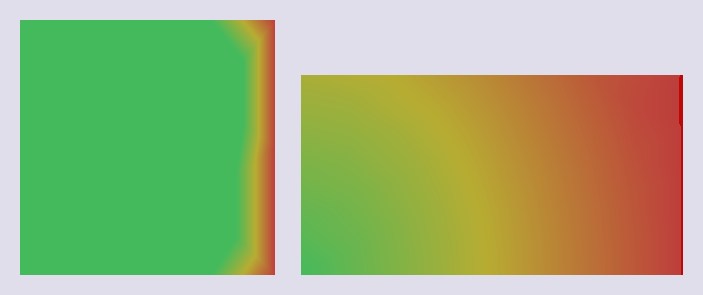
\includegraphics[width=.7\linewidth]{figures/static_analysis}
  \caption{Solution of the static analysis. Left: the initial
condition, right: the solution (deformation magnified 50 times)}
  \label{fig:smm:implicit:static_solution}
\end{figure}


\subsection{Static implicit analysis with dynamic insertion of cohesive elements}
In order to solve problems with the extrinsic cohesive method in the
static implicit solution scheme, the function \code{solveStepCohesive}
has to be used:
\begin{cpp}
model.solveStepCohesive<_scm_newton_raphson_tangent, SolveConvergenceCriteria::_increment>(1e-13, error, 25, false, 1e5, true);
\end{cpp}

in which the arguments are: tolerance, error, max\_iteration,
load\_reduction, tol\_increase\_factor, do\_not\_factorize.  This
function, first applies the Newton-Raphson procedure to solve the
problem.  Then, it calls the method \code{checkCohesiveStress} to
check if cohesive elements have to be inserted.  Since the approach is
implicit, only one element is added, the most stressed one (see
Section \ref{extrinsic_insertion}).  After insertion, the
Newton-Raphson procedure is applied again to solve the same
incremental loading step, with the new inserted cohesive element.  The
procedure loops in this way since no new cohesive elements have to be
inserted.  At that point, the solution is saved, and the simulation
can advance to the next incremental loading step.  In case the
convergence is not reached, the obtained solution is not saved and the
simulation return to the main file with the error given by the
solution saved in the argument of the function \emph{error}.  In this
way, the user can intervene in the simulation in order to find anyhow
convergence.  A possibility is, for instance, to reduce the last
incremental loading step.  The variable \emph{load\_reduction} can be
used to identify if the load has been already reduced or not.  At the
same time, with the variable \emph{tol\_increase\_factor} it is
possible to increase the tolerance by a factor defined by the user in
the main file, in order to accept a solution even with an error bigger
than the tolerance set at the beginning.  It is possible to increase
the tolerance only in the phase of loading reduction, i.e., when
load\_reduction = true.  A not converged solution is never saved.  In
case the convergence is not reached even after the loading reduction
procedure, the displacement field is not updated and remains the one
of the last converged incremental steps.  Also, cohesive elements are
inserted only if convergence is reached.  An example of the extrinsic
cohesive method in the static implicit solution scheme is presented in
\shellcode{\examplesdir/cohesive\_element/cohesive\_extrinsic\_implicit}.

\section{Dynamic Methods} \label{sect:smm:Dynamic_methods}

Different ways to solve the equations of motion are implemented in the
solid mechanics model.  The complete equations that should be solved
are:
\begin{equation}
\label{eqn:equation-motion}
\mat{M}\ddot{\vec{u}} +
\mat{C}\dot{\vec{u}} + \mat{K}\vec{u} = \vec{f}_{\st{ext}}~,
\end{equation}
where $\mat{M}$, $\mat{C}$ and $\mat{K}$ are the mass,
damping and stiffness matrices, respectively.

In the previous section, it has already been discussed how to solve this
equation in the static case, where $\ddot{\vec{u}} = \dot{\vec{u}} = 0$.  Here
the method to solve this equation in the general case will be presented.  For
this purpose, a time discretization has to be specified.  The most common
discretization method in solid mechanics is the Newmark-$\beta$ method, which is
also the default in \akantu.

For the Newmark-$\beta$ method, (\ref{eqn:equation-motion}) becomes a
system of three equations (see \cite{curnier92a} \cite{hughes-83a} for
more details):
\begin{align}
\mat{M} \ddot{\vec{u}}_{n+1} + \mat{C}\dot{\vec{u}}_{n+1} + \mat{K} \vec{u}_{n+1} &={\vec{f}_{\st{ext}}}_{\, n+1}
\label{eqn:equation-motion-discret} \\
\vec{u}_{n+1} &=\vec{u}_{n} + \left(1 - \alpha\right) \Delta t \dot{\vec{u}}_{n} +
\alpha \Delta t \dot{\vec{u}}_{n+1} + \left(\frac{1}{2} -
\alpha\right) \Delta t^2
\ddot{\vec{u}}_{n} \label{eqn:finite-difference-1}\\
\dot{\vec{u}}_{n+1} &= \dot{\vec{u}}_{n} + \left(1 - \beta\right)
\Delta t \ddot{\vec{u}}_{n} + \beta \Delta t
\ddot{\vec{u}}_{n+1} \label{eqn:finite-difference-2}
\end{align}

In these new equations, $\ddot{\vec{u}}_{n}$, $\dot{\vec{u}}_{n}$ and
$\vec{u}_{n}$ are the approximations of $\ddot{\vec{u}}(t_n)$,
$\dot{\vec{u}}(t_n)$ and $\vec{u}(t_n)$.
Equation~(\ref{eqn:equation-motion-discret}) is the equation of motion
discretized in space (finite-element discretization), and equations
(\ref{eqn:finite-difference-1}) and (\ref{eqn:finite-difference-2})
are discretized in both space and time (Newmark discretization).  The
$\alpha$ and $\beta$ parameters determine the stability and the
accuracy of the algorithm. Classical values for $\alpha$ and $\beta$
are usually $\beta = 1/2$ for no numerical damping and $0 < \alpha <
1/2$.

\begin{center}
  \begin{tabular}{cll}
    \toprule
    $\alpha$ & Method ($\beta = 1/2$) & Type\\
    \midrule
    $0$ & central difference & explicit\\
    $1/6$ & Fox-Goodwin (royal road) &implicit\\
    $1/3$ & Linear acceleration &implicit\\
    $1/2$ & Average acceleration (trapezoidal rule)& implicit\\
    \bottomrule
  \end{tabular}
\end{center}

The solution of this system of equations,
(\ref{eqn:equation-motion-discret})-(\ref{eqn:finite-difference-2}) is
split into a predictor and a corrector system of equations.  Moreover,
in the case of a non-linear equations, an iterative algorithm such as
the Newton-Raphson method is applied. The system of equations can be
written as:

\begin{enumerate}
\item \textit{Predictor:}
\begin{align}
  \vec{u}_{n+1}^{0} &= \vec{u}_{n} + \Delta t
  \dot{\vec{u}}_{n} + \frac{\Delta t^2}{2} \ddot{\vec{u}}_{n} \\
  \dot{\vec{u}}_{n+1}^{0} &= \dot{\vec{u}}_{n} + \Delta t
  \ddot{\vec{u}}_{n} \\
  \ddot{\vec{u}}_{n+1}^{0} &= \ddot{\vec{u}}_{n}
\end{align}

\item \textit{Solve:}
\begin{align}
  \left(c \mat{M} + d \mat{C} + e \mat{K}_{n+1}^i\right)
  \vec{w} = {\vec{f}_{\st{ext}}}_{\,n+1} - {\vec{f}_{\st{int}}}_{\,n+1}^i -
  \mat{C} \dot{\vec{u}}_{n+1}^i - \mat{M} \ddot{\vec{u}}_{n+1}^i = \vec{r}_{n+1}^i
\end{align}

\item \textit{Corrector:}
\begin{align}
  \ddot{\vec{u}}_{n+1}^{i+1} &= \ddot{\vec{u}}_{n+1}^{i} +c \vec{w} \\
  \dot{\vec{u}}_{n+1}^{i+1} &= \dot{\vec{u}}_{n+1}^{i} + d\vec{w} \\
  \vec{u}_{n+1}^{i+1} &= \vec{u}_{n+1}^{i} + e \vec{w}
\end{align}
\end{enumerate}

where $i$ is the Newton-Raphson iteration counter and $c$, $d$ and $e$
are parameters depending on the method used to solve the equations

\begin{center}
  \begin{tabular}{lcccc}
    \toprule
    & $\vec{w}$ & $e$ & $d$ & $c$\\
    \midrule
    in acceleration &$ \delta\ddot{\vec{u}}$ & $\alpha \beta\Delta t^2$ &$\beta \Delta t$ &$1$\\
    in velocity & $ \delta\dot{\vec{u}}$& $\alpha\Delta t$ & $1$ & $\frac{1}{\beta \Delta t}$\\
    in displacement &$\delta\vec{u}$ & $ 1$ & $\frac{1}{\alpha \Delta t}$ & $\frac{1}{\alpha \beta \Delta t^2}$\\
    \bottomrule
  \end{tabular}
\end{center}

% \note{If you want to use the implicit solver \akantu should be compiled at
% least with one sparse matrix solver such as Mumps\cite{mumps}.}


\subsection{Implicit Time Integration}
To solve a problem with an implicit time integration scheme, first a
\code{SolidMechanicsModel} object has to be created and initialized.
Then the initial and boundary conditions have to be set.  Everything
is similar to the example in the static case
(Section~\ref{sect:smm:static}), however, in this case the implicit
dynamic scheme is selected at the initialization of the model.

\begin{cpp}
SolidMechanicsModel model(mesh);
model.initFull(_analysis_method = _implicit_dynamic);
/*Boundary conditions see Section ~ %\ref{sect:smm:boundary}% */
\end{cpp}
Because a dynamic simulation is conducted, an integration time step
$\Delta t$ has to be specified. In the case of implicit simulations,
\akantu implements a trapezoidal rule by default.  That is to say
$\alpha = 1/2$ and $\beta = 1/2$ which is unconditionally
stable. Therefore the value of the time step can be chosen arbitrarily
within reason.  \index{SolidMechanicsModel!setTimeStep}
\begin{cpp}
model.setTimeStep(time_step);
\end{cpp}
Since the system has to be solved for a given amount of time steps, the
method \code{solveStep()}, (which has already been used in the static
example in Section~\ref{sect:smm:static}), is called inside a time
loop:
\begin{cpp}
/// time loop
Real time = 0.;

auto & solver = model.getNonLinearSolver();
solver.set("max_iterations", 100);
solver.set("threshold", 1e-12);
solver.set("convergence_type", SolveConvergenceCriteria::_solution);

for (UInt s = 1; time <max_time; ++s, time += time_step) {
  model.solveStep();
}
\end{cpp}
An example of solid mechanics with an implicit time integration scheme
is presented in
\shellcode{\examplesdir/implicit/implicit\_dynamic.cc}.  This example
consists of a 3D beam of
$\SI{10}{\metre}\,\times\,\SI{1}{\metre}\,\times\,\SI{1}{\metre}$
blocked on one side and is on a roller on the other side.  A constant
force of \SI{5}{\kilo\newton} is applied in its middle.
Figure~\ref{fig:smm:implicit:dynamic} presents the geometry of this
case. The material used is a fictitious linear elastic material with a
density of \SI{1000}{\kilo\gram\per\cubic\metre}, a Young's Modulus of
\SI{120}{\mega\pascal} and Poisson's ratio of $0.3$. These values
were chosen to simplify the analytical solution.

An approximation of the dynamic response of the middle point of the
beam is given by:
\begin{equation}
  \label{eqn:smm:implicit}
  u\left(\frac{L}{2}, t\right)
  = \frac{1}{\pi^4} \left(1 - cos\left(\pi^2 t\right) +
    \frac{1}{81}\left(1 - cos\left(3^2 \pi^2 t\right)\right) +
    \frac{1}{625}\left(1 - cos\left(5^2 \pi^2 t\right)\right)\right)
\end{equation}

\begin{figure}[!htb]
  \centering
  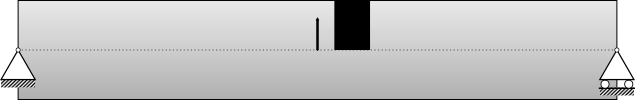
\includegraphics[scale=.6]{figures/implicit_dynamic}
  \caption{Numerical setup}
  \label{fig:smm:implicit:dynamic}
\end{figure}

Figure \ref{fig:smm:implicit:dynamic_solution} presents the deformed
beam at 3 different times during the simulation: time steps 0, 1000 and
2000.

\begin{figure}[!htb]
  \centering
  \setlength{\unitlength}{0.1\textwidth}
  \begin{tikzpicture}
    \node[above right] (img) at (0,0)
    {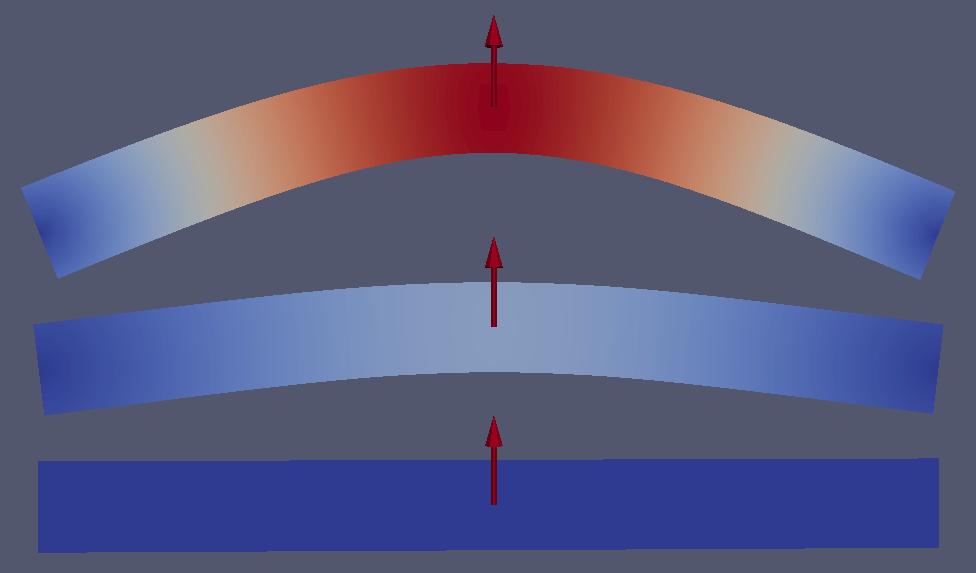
\includegraphics[width=.6\linewidth]{figures/dynamic_analysis}};
    \node[left] at (0pt,20pt) {$0$}; \node[left] at (0pt,60pt) {$1000$};
    \node[left] at (0pt,100pt) {$2000$};
  \end{tikzpicture}

  \caption{Deformed beam at 3 different times (displacement are
    magnified by a factor 10).}
  \label{fig:smm:implicit:dynamic_solution}
\end{figure}

\subsection{Explicit Time Integration}
\label{ssect:smm:expl-time-integr}

The explicit dynamic time integration scheme is based on the
Newmark-$\beta$ scheme with $\alpha=0$ (see equations
\ref{eqn:equation-motion-discret}-\ref{eqn:finite-difference-2}).  In
\akantu, $\beta$ is defaults to $\beta=1/2$, see section
\ref{sect:smm:Dynamic_methods}.

The initialization of the simulation is similar to the static and
implicit dynamic version.  The model is created from the
\code{SolidMechanicsModel} class.  In the initialization, the explicit
scheme is selected using the \code{\_explicit\_lumped\_mass} constant.

\begin{cpp}
SolidMechanicsModel model(mesh);
model.initFull(_analysis_method = _explicit_lumped_mass);
\end{cpp}
\index{SolidMechanicsModel!initFull}
\note{Writing \code{model.initFull()} or \code{model.initFull();} is
equivalent to use the \code{\_explicit\_lumped\_mass} keyword, as this
is the default case.}

The explicit time integration scheme implemented in \akantu uses a
lumped mass matrix $\mat{M}$ (reducing the computational cost). This
matrix is assembled by distributing the mass of each element onto its
nodes. The resulting $\mat{M}$ is therefore a diagonal matrix stored
in the \textbf{mass} vector of the model.

The explicit integration scheme is conditionally stable. The time step
has to be smaller than the stable time step which is obtained in
\akantu as follows:

\begin{cpp}
critical_time_step = model.getStableTimeStep();
\end{cpp} \index{SolidMechanicsModel!StableTimeStep}

The stable time  step corresponds to the time the fastest wave (the compressive
wave) needs to travel the characteristic length of the mesh:
\begin{equation}
\label{eqn:smm:explicit:stabletime}
\Delta t_{\st{crit}} = \frac{\Delta x}{c}
\end{equation}
where $\Delta x$ is a characteristic length (\eg the inradius in the case of
linear triangle element) and $c$ is the celerity of the fastest wave in the
material. It is generally the compressive wave of celerity
$c = \sqrt{\frac{2 \mu + \lambda}{\rho}}$, $\mu$ and $\lambda$ are the first and
second Lame's coefficients and $\rho$ is the density. However, it is recommended
to impose a time step that is smaller than the stable time step, for instance,
by multiplying the stable time step by a safety factor smaller than one.

\begin{cpp}
const Real safety_time_factor = 0.8;
Real applied_time_step = critical_time_step * safety_time_factor;
model.setTimeStep(applied_time_step);
\end{cpp}
\index{SolidMechanicsModel!setTimeStep} The initial displacement and
velocity fields are, by default, equal to zero if not given
specifically by the user (see \ref{sect:smm:initial_condition}).

Like in implicit dynamics, a time loop is used in which the
displacement, velocity and acceleration fields are updated at each
time step. The values of these fields are obtained from the
Newmark$-\beta$ equations with $\beta=1/2$ and $\alpha=0$. In \akantu
these computations at each time step are invoked by calling the
function \code{solveStep}:
\begin{cpp}
for (UInt s = 1; (s-1)*applied_time_step < total_time; ++s) {
  model.solveStep();
}
\end{cpp} \index{SolidMechanicsModel!solveStep}
The method
\code{solveStep} wraps the four following functions:
\begin{itemize}
\item \code{model.explicitPred()} allows to compute the displacement
  field at $t+1$ and a part of the velocity field at $t+1$, denoted by
  $\vec{\dot{u}^{\st{p}}}_{n+1}$, which will be used later in the method
  \code{model.explicitCorr()}. The equations are:
  \begin{align}
    \vec{u}_{n+1} &= \vec{u}_{n} + \Delta t
    \vec{\dot{u}}_{n} + \frac{\Delta t^2}{2} \vec{\ddot{u}}_{n}\\
    \vec{\dot{u}^{\st{p}}}_{n+1} &= \vec{\dot{u}}_{n} + \Delta t
    \vec{\ddot{u}}_{n}
    \label{eqn:smm:explicit:onehalfvelocity}
  \end{align}

\item \code{model.updateResidual()} and
  \code{model.updateAcceleration()} compute the acceleration increment
  $\delta \vec{\ddot{u}}$:
  \begin{equation}
    \left(\mat{M} + \frac{1}{2} \Delta t \mat{C}\right)
    \delta \vec{\ddot{u}} = \vec{f_{\st{ext}}} - \vec{f}_{\st{int}\, n+1}
    - \mat{C} \vec{\dot{u}^{\st{p}}}_{n+1} - \mat{M} \vec{\ddot{u}}_{n}
  \end{equation}

  \note{The internal force $\vec{f}_{\st{int}\, n+1}$ is computed from
    the displacement $\vec{u}_{n+1}$ based on the constitutive law.}

\item \code{model.explicitCorr()} computes the velocity and
  acceleration fields at $t+1$:
  \begin{align}
    \vec{\dot{u}}_{n+1} &= \vec{\dot{u}^{\st{p}}}_{n+1} + \frac{\Delta t}{2}
    \delta \vec{\ddot{u}} \\ \vec{\ddot{u}}_{n+1} &=
    \vec{\ddot{u}}_{n} + \delta \vec{\ddot{u}}
  \end{align}
\end{itemize}

The use of an explicit time integration scheme is illustrated by the
example:\par
\noindent \shellcode{\examplesdir/explicit/explicit\_dynamic.cc}\par
\noindent This example models the propagation of a wave in a steel beam. The
beam and the applied displacement in the $x$ direction are shown in
Figure~\ref{fig:smm:explicit}.

\begin{figure}[!htb] \centering
  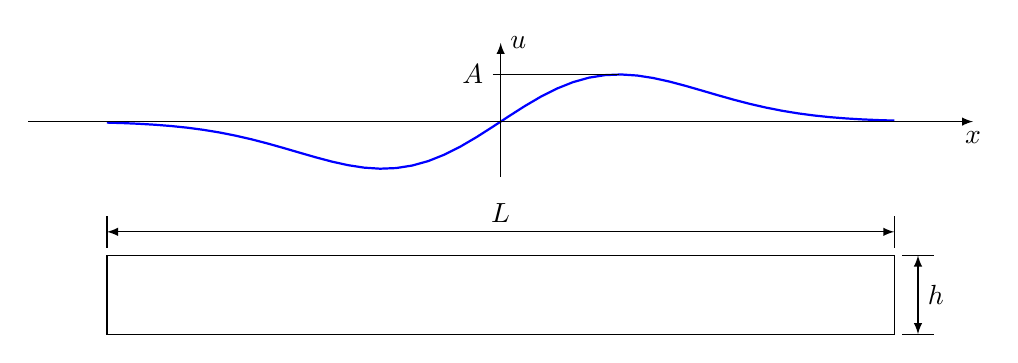
\begin{tikzpicture}
    \coordinate (c) at (0,2);
    \draw[shift={(c)},thick, color=blue] plot [id=x, domain=-5:5, samples=50] ({\x, {(40 * sin(0.1*pi*3*\x) * exp(- (0.1*pi*3*\x)*(0.1*pi*3*\x) / 4))}});
    \draw[shift={(c)},-latex] (-6,0) -- (6,0) node[right, below] {$x$};
    \draw[shift={(c)},-latex] (0,-0.7) -- (0,1) node[right] {$u$};
    \draw[shift={(c)}] (-0.1,0.6) node[left] {$A$}-- (1.5,0.6);

    \coordinate (l) at (0,0.6);
    \draw[shift={(0,-0.7)}] (-5, 0) -- (5,0) -- (5, 1) -- (-5, 1) -- cycle;
    \draw[shift={(l)}, latex-latex] (-5,0)-- (5,0) node [midway, above] {$L$};
    \draw[shift={(l)}] (5,0.2)-- (5,-0.2);
    \draw[shift={(l)}] (-5,0.2)-- (-5,-0.2);

    \coordinate (h) at (5.3,-0.7);
    \draw[shift={(h)}, latex-latex] (0,0)-- (0,1) node [midway, right] {$h$};
    \draw[shift={(h)}] (-0.2,1)-- (0.2,1);
    \draw[shift={(h)}] (-0.2,0)-- (0.2,0);
  \end{tikzpicture}

  \caption{Numerical setup \label{fig:smm:explicit}}
\end{figure}

The length and height of the beam are $L=\SI{10}{\metre}$ and
$h = \SI{1}{\metre}$, respectively.  The material is linear elastic,
homogeneous and isotropic (density:
\SI{7800}{\kilo\gram\per\cubic\metre}, Young's modulus:
\SI{210}{\giga\pascal} and Poisson's ratio: $0.3$).  The imposed
displacement follow a Gaussian function with a maximum amplitude of $A = \SI{0.01}{\meter}$. The
potential, kinetic and total energies are computed.  The safety factor
is equal to $0.8$.

\section{Constitutive Laws \label{sect:smm:CL}}\index{Material}
In order to compute an element's response to deformation, one needs to
use an appropriate constitutive relationship. The constitutive law is
used to compute the element's stresses from the element's strains.

In the finite-element discretization, the constitutive formulation is
applied to every quadrature point of each element. When the implicit
formulation is used, the tangent matrix has to be computed.

The chosen materials for the simulation have to be specified in the
mesh file or, as an alternative, they can be assigned using the
\code{element\_material} vector.  For every material assigned to the
problem one has to specify the material characteristics (constitutive
behavior and material properties) using the text input file (see \ref{sect:io:material}).\\
In order to conveniently store values at each quadrature in a material
point \akantu provides a special data structure, the
\code{InternalField}. The internal fields are inheriting from the
\code{ElementTypeMapArray}.  Furthermore, it provides several functions for
initialization, auto-resizing and auto removal of quadrature points.

Sometimes it is also desired to generate random distributions of
internal parameters. An example might be the critical stress at which the
material fails. To generate such a field, in the text input file,
a random quantity needs be added to the base value:
\begin{cpp}
  sigma_c = $base$
  sigma_c = $base$ uniform [$min$, $max$]
  sigma_c = $base$ weibull [$\lambda$, $m$]
\end{cpp}

All parameters are real numbers. For the uniform distribution, minimum
and maximum values have to be specified.
Random parameters are defined as a $base$ value to which we add a random number
that follows the chosen distribution.

The
\href{http://en.wikipedia.org/wiki/Uniform\_distribution\_(continuous)}{\emph{Uniform}}
distribution is gives a random values between in $[min, max)$. The
\href{http://en.wikipedia.org/wiki/Weibull\_distribution}{\emph{Weibull}}
distribution is characterized by the following cumulative distribution
function:
\begin{equation}
  F(x) = 1- e^{-\left({x/\lambda}\right)^m}
\end{equation}
which depends on  $m$ and $\lambda$, which are the shape parameter and the scale
parameter. These random distributions are different each time the code
is executed. In order to obtain always the same one, it possible to
manually set the \emph{seed} that is the number from which these
pseudo-random distributions are created. This can be done by adding
the following line to the input file \emph{outside} the material
parameters environments:
\begin{cpp}
  seed = 1.0
\end{cpp}
where the value 1 can be substituted with any number. Currently
\akantu is can reproduce always the same distribution when the seed is
specified \emph{only} in serial.

The following sections describe the constitutive models implemented in
\akantu. In Appendix~\ref{app:material-parameters} a summary of the
parameters for all materials of \akantu is provided.


\subsection{Elasticity}\index{Material!Elastic}

The elastic law is a commonly used constitutive relationship that can be used
for a wide range of engineering materials (\eg metals, concrete, rock, wood,
glass, rubber, etc.) provided that the strains remain small (\ie small
deformation and stress lower than yield strength).

The elastic laws are often expressed as $\mat{\sigma} =
\mat{C}:\mat{\varepsilon}$ with where $\mat{\sigma}$ is the Cauchy stress tensor,
$\mat{\varepsilon}$ represents the infinitesimal strain tensor and $\mat{C}$ is the
elastic modulus tensor.

\subsubsection{Linear isotropic\matlabel{ssect:smm:linear-elastic-isotropic}}

The linear isotropic elastic behavior is described by Hooke's law, which states
that the stress is linearly proportional to the applied strain (material behaves
like an ideal spring), as illustrated in Figure~\ref{fig:smm:cl:elastic}.
\begin{figure}[!htb]
  \begin{center}

    \subfloat[]{
      \begin{tikzpicture}
	\draw[thick,latex-latex] (0,5) node[left] {$\sigma$} |- (5,0) node (x) [right, below] {$\varepsilon$};
	\draw[thin] (1.5,1.5) -- (2.5,1.5) -- (2.5,2.5) node [midway, right] {E};
	\draw[very thick,color=red] (0,0) -- (4,4);
	\draw[very thick,latex-latex,color=red] (1,1) -- (3,3);
      \end{tikzpicture}
      \label{fig:smm:cl:elastic:stress_strain} }
    \hspace{0.05\textwidth} \subfloat[]{
      \raisebox{0.125\textwidth}{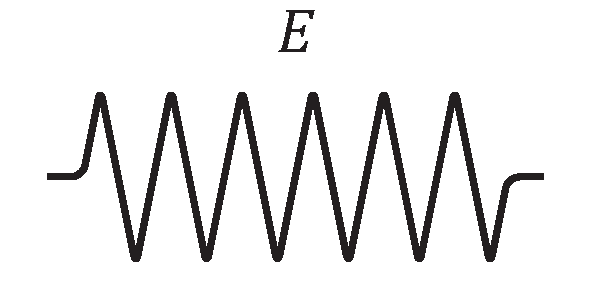
\includegraphics[width=0.25\textwidth,keepaspectratio=true]{figures/hooke_law.pdf}}
      \label{fig:smm:cl:elastic:hooke} }
    \caption{(a) Stress-strain curve for elastic material and (b)
      schematic representation of Hooke's law, denoted as a spring.}
    \label{fig:smm:cl:elastic}
  \end{center}
\end{figure}
The equation that relates the strains to the
displacements is: % First the strain is computed (at every gauss
point) from the displacements as follows:
\begin{equation}
  \label{eqn:smm:strain_inf}
  \mat{\varepsilon} =
  \frac{1}{2} \left[ \nabla_0 \vec{u}+\nabla_0 \vec{u}^T \right]
\end{equation}
where $\mat{\varepsilon}$ represents the infinitesimal strain tensor,
$\nabla_{0}\vec{u}$ the displacement gradient
tensor according to the initial configuration. The constitutive equation
for isotropic homogeneous media can be expressed as:
\begin{equation}
  \label{eqn:smm:material:constitutive_elastic}
  \mat{\sigma } =\lambda\mathrm{tr}(\mat{\varepsilon})\mat{I}+2 \mu\mat{\varepsilon}
\end{equation}
where $\mat{\sigma}$ is the Cauchy stress tensor
($\lambda$ and $\mu$ are the the first and second Lame's
coefficients).

In Voigt notation this correspond to
\begin{align}
  \left[\begin{array}{c}
      \sigma_{11}\\
      \sigma_{22}\\
      \sigma_{33}\\
      \sigma_{23}\\
      \sigma_{13}\\
      \sigma_{12}\\
    \end{array}\right]
  &= \frac{E}{(1+\nu)(1-2\nu)}\left[
    \begin{array}{cccccc}
      1-\nu & \nu   & \nu   & 0 & 0 & 0\\
      \nu   & 1-\nu & \nu   & 0 & 0 & 0\\
      \nu   & \nu   & 1-\nu & 0 & 0 & 0\\
      0     &  0    &  0    & \frac{1-2\nu}{2} & 0 & 0 \\
      0     &  0    &  0    & 0 & \frac{1-2\nu}{2} & 0 \\
      0     &  0    &  0    & 0 & 0 & \frac{1-2\nu}{2} \\
    \end{array}\right]
  \left[\begin{array}{c}
      \varepsilon_{11}\\
      \varepsilon_{22}\\
      \varepsilon_{33}\\
      2\varepsilon_{23}\\
      2\varepsilon_{13}\\
      2\varepsilon_{12}\\
    \end{array}\right]
\end{align}

\subsubsection{Linear anisotropic\matlabel{ssect:smm:linear-elastic-anisotropic}}
This formulation is not sufficient to represent all elastic material
behavior. Some materials have characteristic orientation that have to be taken
into account. To represent this anisotropy a more general stress-strain law has
to be used. For this we define the elastic modulus tensor as follow:

\begin{align}
  \left[\begin{array}{c}
      \sigma_{11}\\
      \sigma_{22}\\
      \sigma_{33}\\
      \sigma_{23}\\
      \sigma_{13}\\
      \sigma_{12}\\
    \end{array}\right]
  &= \left[
    \begin{array}{cccccc}
      c_{11} & c_{12} & c_{13} & c_{14} & c_{15} & c_{16}\\
      c_{21} & c_{22} & c_{23} & c_{24} & c_{25} & c_{26}\\
      c_{31} & c_{32} & c_{33} & c_{34} & c_{35} & c_{36}\\
      c_{41} & c_{42} & c_{43} & c_{44} & c_{45} & c_{46}\\
      c_{51} & c_{52} & c_{53} & c_{54} & c_{55} & c_{56}\\
      c_{61} & c_{62} & c_{63} & c_{64} & c_{65} & c_{66}\\
    \end{array}\right]
  \left[\begin{array}{c}
      \varepsilon_{11}\\
      \varepsilon_{22}\\
      \varepsilon_{33}\\
      2\varepsilon_{23}\\
      2\varepsilon_{13}\\
      2\varepsilon_{12}\\
    \end{array}\right]
\end{align}

\begin{figure}[h]
  \centering
  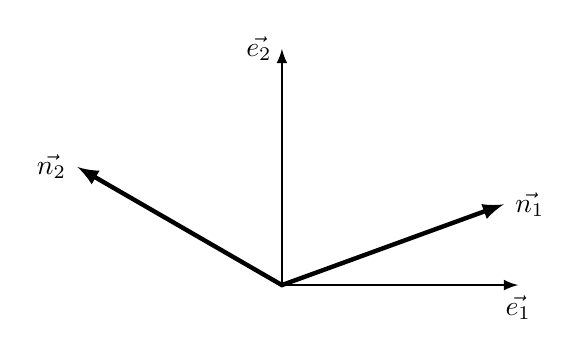
\begin{tikzpicture}
    \draw[thick,latex-latex] (90:3) node[left] {$\vec{e_2}$} |- (0:3) node [right, below] {$\vec{e_1}$};
    \draw[ultra thick,latex-latex] (150:3) node[left] {$\vec{n_2}$} -- (0,0) -- (20:3) node [right] {$\vec{n_1}$};
  \end{tikzpicture}
  \caption{Material basis}
\end{figure}

To simplify the writing of input files the \mat{C} tensor is expressed in the
material basis. And this basis as to be given too. This basis $\Omega_{\st{mat}}
= \{\vec{n_1}, \vec{n_2}, \vec{n_3}\}$ is used to define the rotation $R_{ij} =
\vec{n_j} . \vec{e_i}$. And $\mat{C}$ can be rotated in the global basis $\Omega
= \{\vec{e_1}, \vec{e_2}, \vec{e_3}\}$ as follow:


\begin{align}
\mat{C}_{\Omega} &= \mat{R}_1 \mat{C}_{\Omega_{\st{mat}}} \mat{R}_2\\
\mat{R}_1  &= \left[
  \begin{array}{cccccc}
    R_{11} R_{11} & R_{12} R_{12} & R_{13} R_{13} & R_{12} R_{13} & R_{11} R_{13} & R_{11} R_{12}\\
    R_{21} R_{21} & R_{22} R_{22} & R_{23} R_{23} & R_{22} R_{23} & R_{21} R_{23} & R_{21} R_{22}\\
    R_{31} R_{31} & R_{32} R_{32} & R_{33} R_{33} & R_{32} R_{33} & R_{31} R_{33} & R_{31} R_{32}\\
    R_{21} R_{31} & R_{22} R_{32} & R_{23} R_{33} & R_{22} R_{33} & R_{21} R_{33} & R_{21} R_{32}\\
    R_{11} R_{31} & R_{12} R_{32} & R_{13} R_{33} & R_{12} R_{33} & R_{11} R_{33} & R_{11} R_{32}\\
    R_{11} R_{21} & R_{12} R_{22} & R_{13} R_{23} & R_{12} R_{23} & R_{11} R_{23} & R_{11} R_{22}\\
  \end{array}\right]\\
\mat{R}_2  &= \left[
  \begin{array}{cccccc}
    R_{11} R_{11} & R_{21} R_{21} & R_{31} R_{31} & R_{21} R_{31} & R_{11} R_{31} & R_{11} R_{21}\\
    R_{12} R_{12} & R_{22} R_{22} & R_{32} R_{32} & R_{22} R_{32} & R_{12} R_{32} & R_{12} R_{22}\\
    R_{13} R_{13} & R_{23} R_{23} & R_{33} R_{33} & R_{23} R_{33} & R_{13} R_{33} & R_{13} R_{23}\\
    R_{12} R_{13} & R_{22} R_{23} & R_{32} R_{33} & R_{22} R_{33} & R_{12} R_{33} & R_{12} R_{23}\\
    R_{11} R_{13} & R_{21} R_{23} & R_{31} R_{33} & R_{21} R_{33} & R_{11} R_{33} & R_{11} R_{23}\\
    R_{11} R_{12} & R_{21} R_{22} & R_{31} R_{32} & R_{21} R_{32} & R_{11} R_{32} & R_{11} R_{22}\\
  \end{array}\right]\\
\end{align}

\subsubsection{Linear orthotropic\matlabel{ssect:smm:linear-elastic-orthotropic}}

A particular case of anisotropy is when the material basis is orthogonal in which case the elastic modulus tensor can be simplified and rewritten in terms of 9 independents material parameters.

\begin{align}
  \left[\begin{array}{c}
      \sigma_{11}\\
      \sigma_{22}\\
      \sigma_{33}\\
      \sigma_{23}\\
      \sigma_{13}\\
      \sigma_{12}\\
    \end{array}\right]
  &= \left[
    \begin{array}{cccccc}
      c_{11} & c_{12} & c_{13} &   0   &   0   &   0  \\
            & c_{22} & c_{23} &   0   &   0   &   0  \\
            &       & c_{33} &   0   &   0   &   0  \\
            &       &       & c_{44} &   0   &   0  \\
            &  \multicolumn{2}{l}{\text{sym.}}       &       & c_{55} &   0  \\
            &       &       &       &       & c_{66}\\
    \end{array}\right]
  \left[\begin{array}{c}
      \varepsilon_{11}\\
      \varepsilon_{22}\\
      \varepsilon_{33}\\
      2\varepsilon_{23}\\
      2\varepsilon_{13}\\
      2\varepsilon_{12}\\
    \end{array}\right]
\end{align}

\begin{align}
  c_{11} &= E_1 (1 - \nu_{23}\nu_{32})\Gamma \qquad c_{22} = E_2 (1 - \nu_{13}\nu_{31})\Gamma \qquad c_{33} = E_3 (1 - \nu_{12}\nu_{21})\Gamma\\
  c_{12} &= E_1 (\nu_{21} - \nu_{31}\nu_{23})\Gamma = E_2 (\nu_{12} - \nu_{32}\nu_{13})\Gamma\\
  c_{13} &= E_1 (\nu_{31} - \nu_{21}\nu_{32})\Gamma = E_2 (\nu_{13} - \nu_{21}\nu_{23})\Gamma\\
  c_{23} &= E_2 (\nu_{32} - \nu_{12}\nu_{31})\Gamma = E_3 (\nu_{23} - \nu_{21}\nu_{13})\Gamma\\
  c_{44} &= \mu_{23} \qquad  c_{55} = \mu_{13} \qquad  c_{66} = \mu_{12} \\
  \Gamma &= \frac{1}{1 - \nu_{12} \nu_{21} - \nu_{13} \nu_{31} - \nu_{32} \nu_{23} - 2 \nu_{21} \nu_{32} \nu_{13}}
\end{align}

The Poisson ratios follow the rule $\nu_{ij} = \nu_{ji} E_i / E_j$.

\subsection{Neo-Hookean\matlabel{ssect:smm:cl:neohookean}}\index{Material!Neohookean}
The hyperelastic Neo-Hookean constitutive law results from an
extension of the linear elastic relationship (Hooke's Law) for large
deformation. Thus, the model predicts nonlinear stress-strain behavior
for bodies undergoing large deformations.

\begin{figure}[!htb]
  \begin{center}
    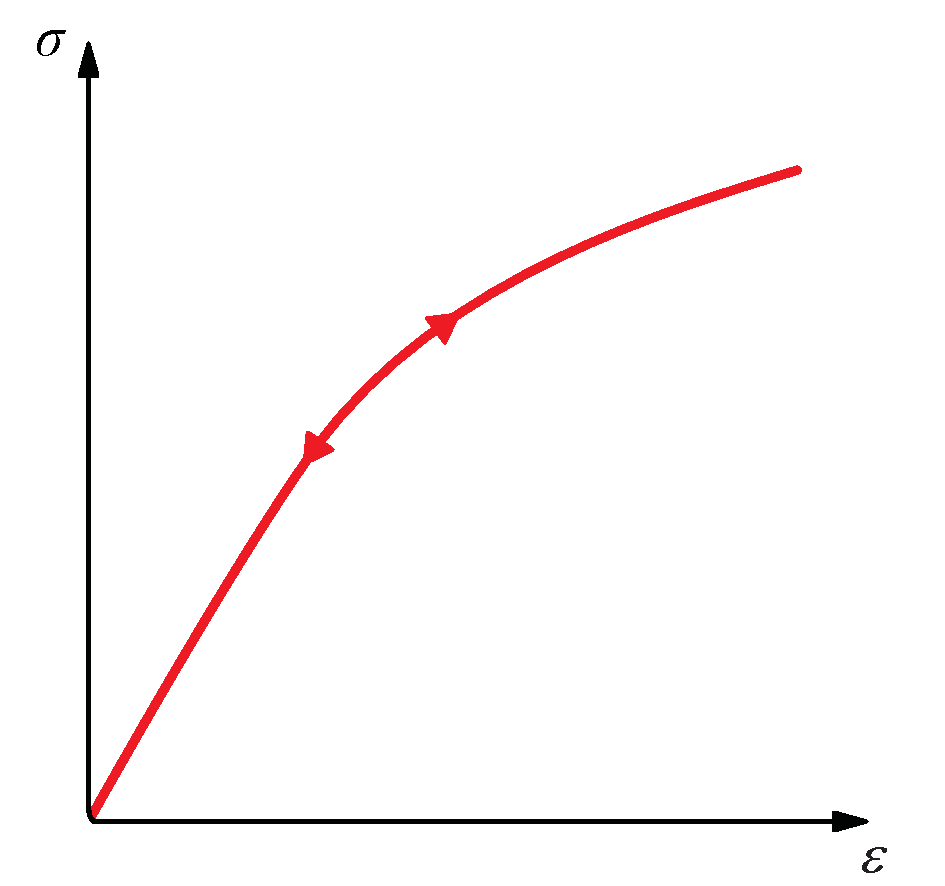
\includegraphics[width=0.4\textwidth,keepaspectratio=true]{figures/stress_strain_neo.pdf}
    \caption{Neo-hookean Stress-strain curve.}
    \label{fig:smm:cl:neo_hookean}
  \end{center}
\end{figure}

As illustrated in Figure~\ref{fig:smm:cl:neo_hookean}, the behavior is initially
linear and the mechanical behavior is very close to the corresponding linear
elastic material. This constitutive relationship, which accounts for compressibility,
is a modified version of the one proposed by Ronald Rivlin \cite{Belytschko:2000}.

The strain energy stored in the material is given by:
\begin{equation}\label{eqn:smm:constitutive:neohookean_potential}
  \Psi(\mat{C}) = \frac{1}{2}\lambda_0\left(\ln J\right)^2-\mu_0\ln J+\frac{1}{2}
  \mu_0\left(\mathrm{tr}(\mat{C})-3\right)
\end{equation}
\noindent where $\lambda_0$ and $\mu_0$ are, respectively, Lam\'e's first parameter
and the shear modulus at the initial configuration. $J$ is the jacobian of the deformation
gradient ($\mat{F}=\nabla_{\!\!\vec{X}}\vec{x}$): $J=\text{det}(\mat{F})$. Finally $\mat{C}$ is the right Cauchy-Green
deformation tensor.

Since this kind of material is used for large deformation problems, a
finite deformation framework should be used. Therefore, the Cauchy
stress ($\mat{\sigma}$) should be computed through the second
Piola-Kirchhoff stress tensor $\mat{S}$:

\begin{equation}
  \mat{\sigma } = \frac{1}{J}\mat{F}\mat{S}\mat{F}^T
\end{equation}

Finally the second Piola-Kirchhoff stress tensor is given by:

\begin{equation}
  \mat{S}  = 2\frac{\partial\Psi}{\partial\mat{C}} = \lambda_0\ln J
  \mat{C}^{-1}+\mu_0\left(\mat{I}-\mat{C}^{-1}\right)
\end{equation}

The parameters to indicate in the material file are the same
as those for the elastic case: \code{E} (Young's modulus), \code{nu} (Poisson's
ratio).


\subsection{Visco-Elasticity\matlabel{ssect:smm:cl:sls}}
% Standard Solid rheological model, see [] J.C. Simo, T.J.R. Hughes,
% "Computational Inelasticity", Springer (1998), see Sections 10.2 and 10.3
Visco-elasticity is characterized by strain rate dependent
behavior. Moreover, when such a material undergoes a deformation it
dissipates energy. This dissipation results in a hysteresis loop in
the stress-strain curve at every loading cycle (see
Figure~\ref{fig:smm:cl:visco-elastic:hyst}). In principle, it can be
applied to many materials, since all materials exhibit a visco-elastic
behavior if subjected to particular conditions (such as high
temperatures).
\begin{figure}[!htb]
  \begin{center}

    \subfloat[]{
      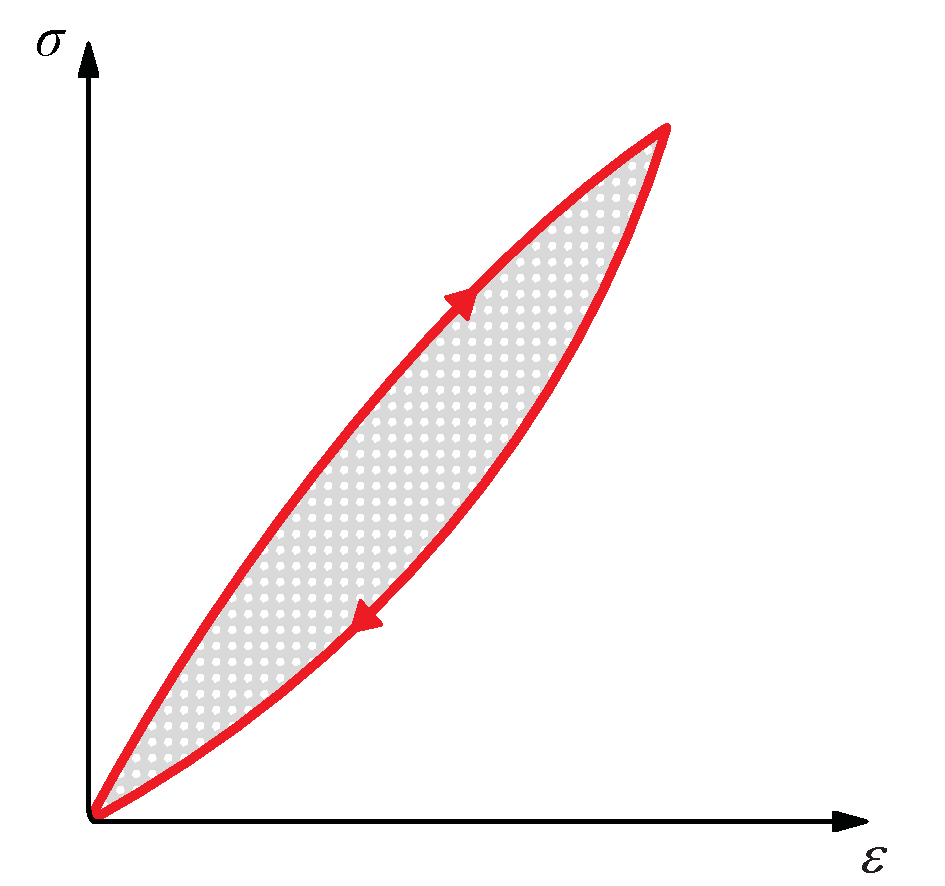
\includegraphics[width=0.4\textwidth,keepaspectratio=true]{figures/stress_strain_visco.pdf}
      \label{fig:smm:cl:visco-elastic:hyst}
    }
    \hspace{0.05\textwidth}
    \subfloat[]{
      \raisebox{0.025\textwidth}{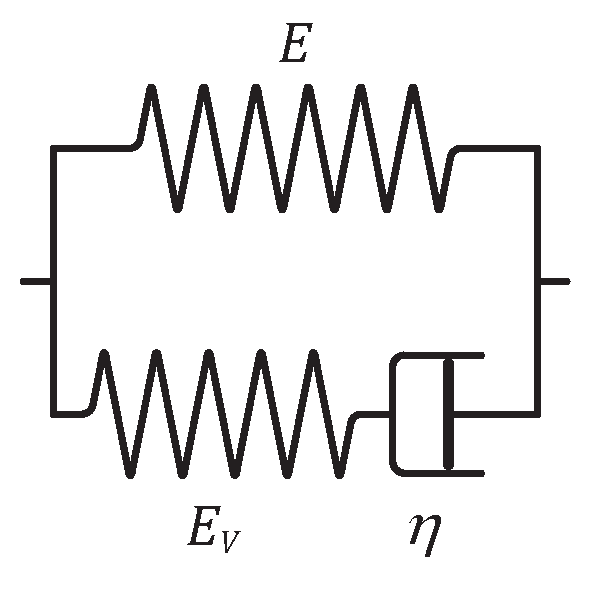
\includegraphics[width=0.3\textwidth,keepaspectratio=true]{figures/visco_elastic_law.pdf}}
      \label{fig:smm:cl:visco-elastic:model}
    }
    \caption{(a) Characteristic stress-strain behavior of a visco-elastic material with hysteresis loop and (b) schematic representation of the standard rheological linear solid visco-elastic model.}
    \label{fig:smm:cl:visco-elastic}
  \end{center}
\end{figure}
The standard rheological linear solid model (see Sections 10.2 and 10.3
of~\cite{simo92}) has been implemented in \akantu. This model results from the
combination of a spring mounted in parallel with a spring and a dashpot
connected in series, as illustrated in
Figure~\ref{fig:smm:cl:visco-elastic:model}. The advantage of this model is that
it allows to account for creep or stress relaxation. The equation that relates
the stress to the strain is (in 1D):
\begin{equation}
  \frac{d\varepsilon(t)}{dt} = \left ( E + E_V \right ) ^ {-1} \cdot \left [ \frac{d\sigma(t)}{dt} + \frac{E_V}{\eta}\sigma(t) - \frac{EE_V}{\eta}\varepsilon(t) \right ]
\end{equation}
where $\eta$ is the viscosity. The equilibrium condition is unique and
is attained in the limit, as $t \to \infty $. At this stage, the
response is elastic and depends on the Young's modulus $E$.  The
mandatory parameters for the material file are the following:
\code{rho} (density), \code{E} (Young's modulus), \code{nu} (Poisson's
ratio), \code{Plane\_Stress} (if set to zero plane strain, otherwise
plane stress), \code{eta} (dashpot viscosity) and \code{Ev} (stiffness
of the viscous element).

Note that the current standard linear solid model is applied only on the deviatoric part of the strain tensor. The spheric part of the strain tensor affects the stress tensor like an linear elastic material.

\subsection{Small-Deformation Plasticity\matlabel{ssect:smm:cl:plastic}}\index{Material!Small-deformation Plasticity}
The small-deformation plasticity is a simple plasticity material
formulation which accounts for the additive decomposition of strain
into elastic and plastic strain components. This formulation is
applicable to infinitesimal deformation where the additive
decomposition of the strain is a valid approximation. In this
formulation, plastic strain is a shearing process where hydrostatic
stress has no contribution to plasticity and consequently plasticity
does not lead to volume change. Figure~\ref{fig:smm:cl:Lin-strain-hard}
shows the linear strain hardening elasto-plastic behavior according to
the additive decomposition of strain into the elastic and plastic
parts in infinitesimal deformation as
\begin{align}
  \mat{\varepsilon} &= \mat{\varepsilon}^e +\mat{\varepsilon}^p\\
  {\mat{\sigma}} &= 2G(\mat{\varepsilon}^e) + \lambda  \mathrm{tr}(\mat{\varepsilon}^e)\mat{I}
\end{align}

\begin{figure}[htp]
  \centering
  {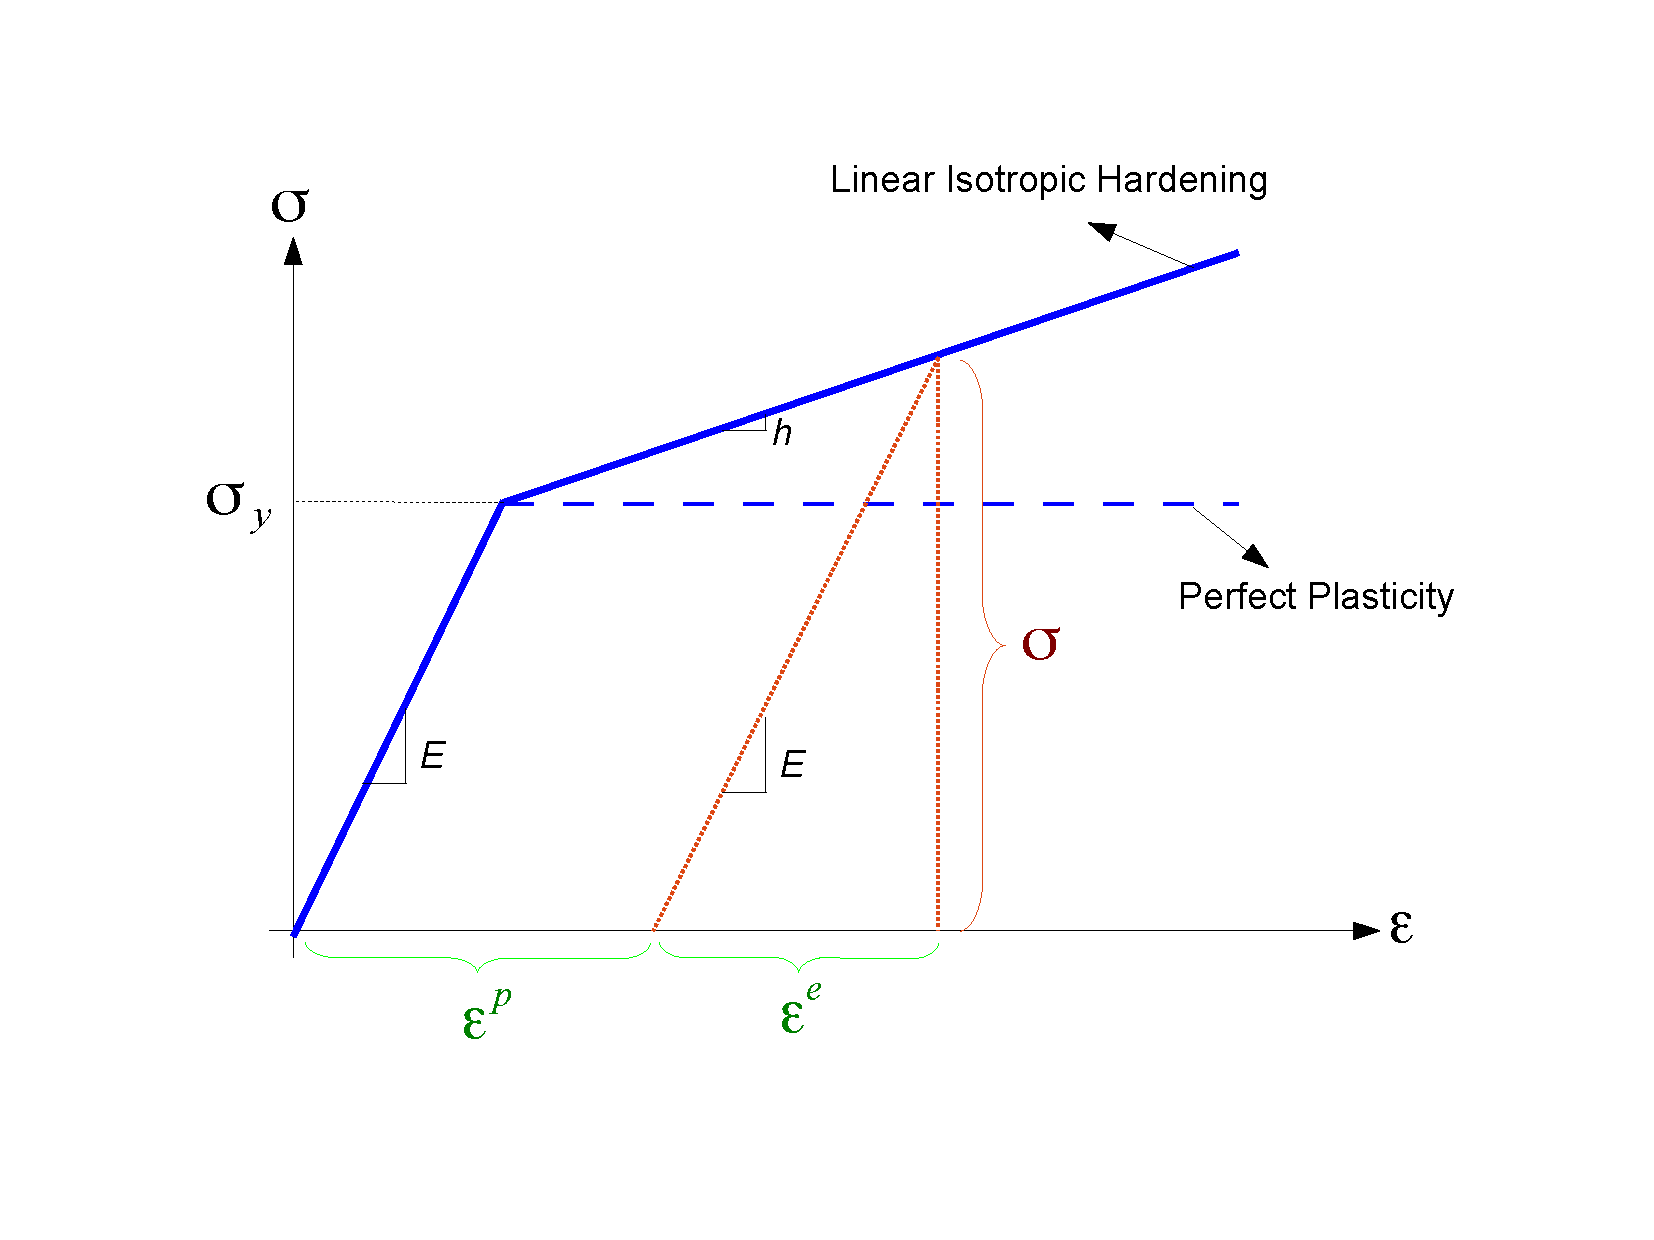
\includegraphics[scale=0.4, clip]{figures/isotropic_hardening_plasticity.pdf}}
  \caption{
    Stress-strain curve for the small-deformation plasticity with linear isotropic hardening.
  }
  \label{fig:smm:cl:Lin-strain-hard}
\end{figure}

\noindent In this class, the von Mises yield criterion is used. In the von Mises yield criterion, the yield is independent of the hydrostatic stress. Other yielding criteria such as Tresca and Gurson can be easily implemented in this class as well.

In the von Mises yield criterion, the hydrostatic stresses have no effect on the plasticity and consequently the yielding occurs when a critical elastic shear energy is achieved.
\begin{equation} \label{eqn:smm:constitutive:von Mises}
  f = \sigma_{\st{eff}} - \sigma_y = \left(\frac{3}{2} {\mat{\sigma}}^{\st{tr}} : {\mat{\sigma}}^{\st{tr}}\right)^\frac{1}{2}-\sigma_y (\mat{\varepsilon}^p)
\end{equation}
\begin{equation} \label{eqn:smm:constitutive:yielding}
  f < 0 \quad \textrm{Elastic deformation,} \qquad f = 0 \quad  \textrm{Plastic deformation}
\end{equation}
where $\sigma_y$ is the yield strength of the material which can be function of plastic strain in case of hardening type of materials and ${\mat{\sigma}}^{\st{tr}}$ is the deviatoric part of stress given by
\begin{equation} \label{eqn:smm:constitutive:deviatoric stress}
  {\mat{\sigma}}^{\st{tr}}=\mat{\sigma} - \frac{1}{3} \mathrm{tr}(\mat{\sigma}) \mat {I}
\end{equation}

After yielding $(f = 0)$, the normality hypothesis of plasticity determines the direction of plastic flow which is normal to the tangent to the yielding surface at the load point. Then, the tensorial form of the plastic constitutive equation using the von Mises yielding criterion (see equation 4.34) may be written as
\begin{equation} \label{eqn:smm:constitutive:plastic contitutive equation}
  \Delta {\mat{\varepsilon}}^p = \Delta p \frac {\partial{f}}{\partial{\mat \sigma}}=\frac{3}{2} \Delta p \frac{{\mat{\sigma}}^{\st{tr}}}{\sigma_{\st{eff}}}
\end{equation}

In these expressions, the direction of the plastic strain increment (or equivalently, plastic strain rate) is given by $\frac{{\mat{\sigma}}^{\st{tr}}}{\sigma_{\st{eff}}}$ while the magnitude is defined by the plastic multiplier $\Delta p$. This can be obtained using the \emph{consistency condition} which impose the requirement for the load point to remain on the yielding surface in the plastic regime.

Here, we summarize the implementation procedures for the
small-deformation plasticity with linear isotropic hardening:
\begin{enumerate}
\item Compute the trial stress:
  \begin{equation}
    {\mat{\sigma}}^{\st{tr}} = {\mat{\sigma}}_t + 2G\Delta \mat{\varepsilon} + \lambda \mathrm{tr}(\Delta \mat{\varepsilon})\mat{I}
  \end{equation}
\item Check the Yielding criteria:
  \begin{equation}
    f = (\frac{3}{2} {\mat{\sigma}}^{\st{tr}} : {\mat{\sigma}}^{\st{tr}})^{1/2}-\sigma_y (\mat{\varepsilon}^p)
  \end{equation}
\item Compute the Plastic multiplier:
  \begin{align}
    d \Delta p &= \frac{\sigma^{tr}_{eff} - 3G \Delta P^{(k)}- \sigma_y^{(k)}}{3G + h}\\
    \Delta p^{(k+1)} &= \Delta p^{(k)}+ d\Delta p\\
    \sigma_y^{(k+1)} &= (\sigma_y)_t+ h\Delta p
  \end{align}
\item Compute the plastic strain increment:
  \begin{equation}
    \Delta {\mat{\varepsilon}}^p = \frac{3}{2} \Delta p \frac{{\mat{\sigma}}^{\st{tr}}}{\sigma_{\st{eff}}}
  \end{equation}
\item Compute the stress increment:
  \begin{equation}
    {\Delta \mat{\sigma}} = 2G(\Delta \mat{\varepsilon}-\Delta \mat{\varepsilon}^p) + \lambda  \mathrm{tr}(\Delta \mat{\varepsilon}-\Delta \mat{\varepsilon}^p)\mat{I}
  \end{equation}
\item Update the variables:
  \begin{align}
    {\mat{\varepsilon^p}} &= {\mat{\varepsilon}}^p_t+{\Delta {\mat{\varepsilon}}^p}\\
    {\mat{\sigma}} &= {\mat{\sigma}}_t+{\Delta \mat{\sigma}}
  \end{align}
\end{enumerate}

We use an implicit integration technique called \emph{the radial
  return method} to obtain the plastic multiplier. This method has the
advantage of being unconditionally stable, however, the accuracy
remains dependent on the step size. The plastic parameters to indicate
in the material file are: \code{$\sigma_y$} (Yield stress) and
\code{h} (Hardening modulus). In addition, the elastic parameters need
to be defined as previously mentioned: \code{E} (Young's modulus),
\code{nu} (Poisson's ratio).

\subsection{Damage}

In the  simplified case of a  linear elastic and brittle  material, isotropic
damage can be represented by a scalar variable $d$, which varies from $0$ to $1$
for  no  damage  to  fully  broken  material  respectively.  The  stress-strain
relationship then becomes:
\begin{equation*}
  \mat{\sigma} = (1-d)\, \mat{C}:\mat{\varepsilon}
\end{equation*}

where  $\mat{\sigma}$,  $\mat{\varepsilon}$ are  the  Cauchy  stress and  strain
tensors, and $\mat{C}$ is the elastic stiffness tensor. This formulation relies
on the definition of an evolution law for the damage variable. In \akantu, many
possibilities exist and they are listed below.

\subsubsection{Marigo\matlabel{ssect:smm:cl:damage-marigo}}

This damage evolution law is energy based as defined by Marigo \cite{marigo81a,
  lemaitre96a}. It is an isotropic damage law.
\begin{align}
  Y &= \frac{1}{2}\mat{\varepsilon}:\mat{C}:\mat{\varepsilon}\\
  F &= Y - Y_d - S d\\
  d &= \left\{
    \begin{array}{l l}
      \mathrm{min}\left(\frac{Y-Y_d}{S},\;1\right) & \mathrm{if}\; F > 0\\
      \mathrm{unchanged} & \mathrm{otherwise}
    \end{array}
  \right.
\end{align}
In this formulation, $Y$ is the strain energy release rate, $Y_d$ the
rupture criterion and $S$ the damage energy.  The non-local version of
this damage evolution law is constructed by averaging the energy $Y$.

\subsubsection{Mazars\matlabel{ssect:smm:cl:damage-mazars}}

This law introduced by Mazars \cite{mazars84a} is a behavioral model to
represent damage evolution in concrete. This model does not rely on the computation of the tangent stiffness, the damage is directly evaluated from the strain.

The governing variable in this damage
law is the equivalent strain $\varepsilon_{\st{eq}} =
\sqrt{<\mat{\varepsilon}>_+:<\mat{\varepsilon}>_+}$, with $<.>_+$ the positive
part of the tensor. This part is defined in the principal coordinates (I, II, III) as $\varepsilon_{\st{eq}} =
\sqrt{<\mat{\varepsilon_I}>_+^2 + <\mat{\varepsilon_{II}}>_+^2 + <\mat{\varepsilon_{III}}>_+^2}$.
The damage is defined as:
\begin{align}
  D &= \alpha_t^\beta D_t + (1-\alpha_t)^\beta D_c\\
  D_t &= 1 - \frac{\kappa_0 (1- A_t)}{\varepsilon_{\st{eq}}} - A_t \exp^{-B_t(\varepsilon_{\st{eq}}-\kappa_0)}\\
  D_c &= 1 - \frac{\kappa_0 (1- A_c)}{\varepsilon_{\st{eq}}} - A_c
  \exp^{-B_c(\varepsilon_{\st{eq}}-\kappa_0)}\\
  \alpha_t &= \frac{\sum_{i=1}^3<\varepsilon_i>_+\varepsilon_{\st{nd}\;i}}{\varepsilon_{\st{eq}}^2}
\end{align}
With $\kappa_0$ the damage threshold, $A_t$ and $B_t$ the damage parameter in
traction, $A_c$ and $B_c$ the damage parameter in compression, $\beta$ is the
shear parameter. $\alpha_t$ is the coupling parameter between traction and
compression, the $\varepsilon_i$ are the eigenstrain and the
$\varepsilon_{\st{nd}\;i}$ are the eigenvalues of the strain if the material
were undamaged.

The coefficients $A$ and $B$ are the post-peak asymptotic
value and the decay shape parameters.

\IfFileExists{manual-constitutive-laws-non_local.tex}{\section{Non-Local Constitutive Laws \label{sect:smm:CLNL}}\index{Material}

Continuum damage modeling of quasi-brittle materials undergo significant softening after the onset of damage. This fast growth of damage causes a loss of ellipticity of partial differential equations of equilibrium. Therefore, the numerical simulation results won't be objective anymore, because the dissipated energy will depend on mesh size used in the simulation. One way to avoid this effect is the use of non-local damage formulations. In this approach a local quantity such as the strain is replaced by its non-local average, where the size of the domain, over which the quantitiy is averaged, depends on the underlying material microstructure. 
\akantu provides non-local versions of many constitutive laws for damage. Examples are for instance the material Mazar and the material Marigo, that can be used in a non-local context. In order to use the corresponding non-local formulation the user has to define the non-local material he wishes to use in the text input file:
\begin{cpp}
  material %\emph{constitutive\_law\_non\_local}% [
     name = %\emph{material\_name}
     rho = $value$
     ...
  ]
\end{cpp}
where \emph{constitutive\_law\_non\_local} is the name of the non-local consitutive law, \textit{e.g.} \emph{marigo\_non\_local}.
In addition to the material the non-local neighborhood, that should be used for the averaging process needs to be defined in the material file as well: 
\begin{cpp}
  non_local %\emph{neighborhood\_name}%  %\emph{weight\_function\_type}% [
     radius = $value$
     ...
      weight_function weight_parameter [
        damage_limit = $value$
        ...
     ]
  ]
\end{cpp}
for the non-local averaging, \textit{e.g.} \emph{base\_wf}, followed by the properties of the non-local neighborhood, such as the radius, and the weight function parameters. It is important to notice that the non-local neighborhood must have the same name as the material to which the neighborhood belongs!
The following two sections list the non-local constitutive laws and different type of weight functions available in \akantu.
\subsection{Non-local constitutive laws}
\textbf{Description to be added!!!}
\subsection{Non-local weight functions}
 \textbf{Description to be added!!!}}{}

\IfFileExists{manual-extra_materials.tex}{% \subsubsection{Caughey}
% ** Not in  release ** The model  is a particular case of  the Rayleigh damping
% model,   with    damping   being   proportional   only    to   the   stiffness
% matrix. Substitute with complete Rayleigh damping model for release?

\subsection{Neo-Hookean}\index{Material!Neohookean}

The hyperelastic Neo-Hookean constitutive law results from an
extension of the linear elastic relationship (Hooke's Law) for large
deformation. Thus, the model predicts nonlinear stress-strain behavior
for bodies undergoing large deformations.

\begin{figure}[!htb]
  \begin{center}
    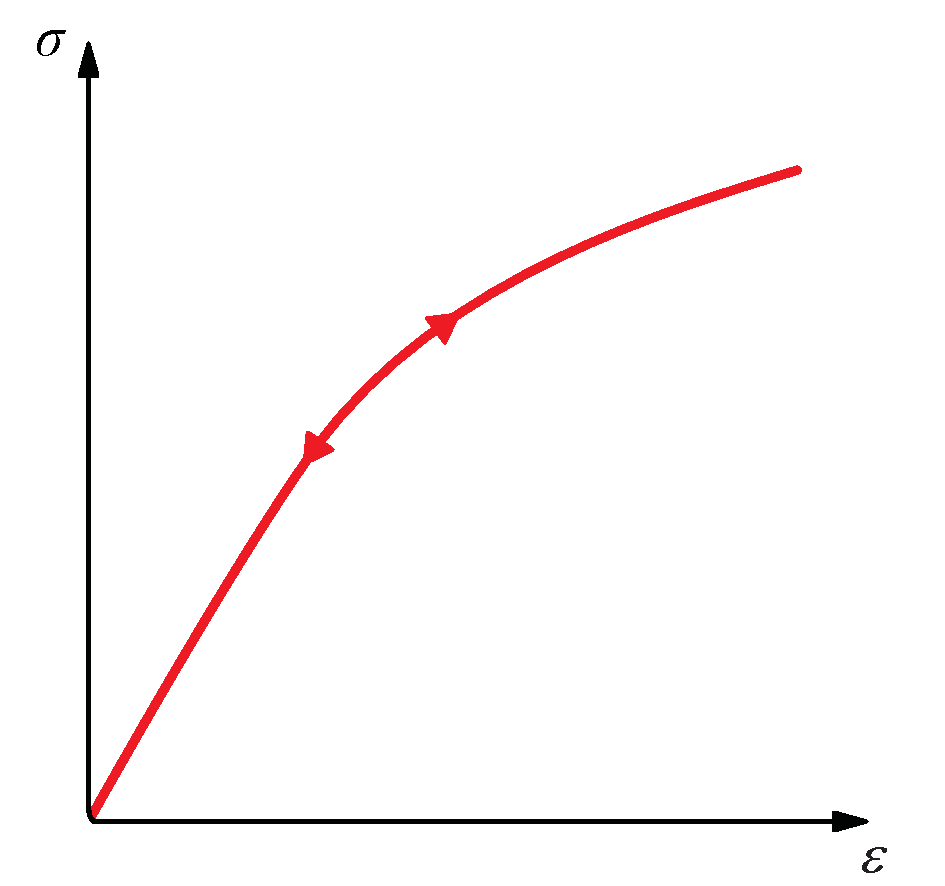
\includegraphics[width=0.4\textwidth,keepaspectratio=true]{figures/stress_strain_neo.pdf}
    \caption{Neo-hookean Stress-strain curve.}
    \label{fig:smm:cl:neo_hookean}
  \end{center}
\end{figure}

As illustrated in Figure~\ref{fig:smm:cl:neo_hookean}, the behavior is initially
linear and the mechanical behavior is very close to the corresponding linear
elastic material. This constitutive relationship, which accounts for compressibility,
 is a modified version of the one proposed by Ronald Rivlin \cite{Belytschko:2000}.

The strain energy stored in the material is given by:
\begin{equation}\label{eqn:smm:constitutive:neohookean_potential}
  \Psi(\mat{C}) = \frac{1}{2}\lambda_0\left(\ln J\right)^2-\mu_0\ln J+\frac{1}{2}
\mu_0\left(\text{trace}(\mat{C})-3\right)
\end{equation}
\noindent where $\lambda_0$ and $\mu_0$ are, respectively, Lamé's first parameter
and the shear modulus at the initial configuration. $J$ is the jacobian of the deformation
gradient ($\mat{F}=\nabla_{\!\!\vec{X}}\vec{x}$): $J=\text{det}(\mat{F})$. Finally $\mat{C}$ is the right Cauchy-Green
deformation tensor.

Since this kind of material is used for large deformation problems, a
finite deformation framework should be used. Therefore, the Cauchy
stress ($\mat{\sigma}$) should be computed through the second
Piola-Kirchhoff stress tensor $\mat{S}$:

\begin{equation}
  \mat{\sigma } = \frac{1}{J}\mat{F}\mat{S}\mat{F}^T
\end{equation}

Finally the second Piola-Kirchhoff stress tensor is given by:

\begin{equation}
  \mat{S}  = 2\frac{\partial\Psi}{\partial\mat{C}} = \lambda_0\ln J
\mat{C}^{-1}+\mu_0\left(\mat{I}-\mat{C}^{-1}\right)
\end{equation}

The parameters to indicate in the material file are the same
as those for the elastic case: \code{E} (Young's modulus), \code{nu} (Poisson's
ratio).

\subsection{Small-Deformation Plasticity}\index{Material!Small-deformation Plasticity}


The small-deformation plasticity is a simple plasticity material
formulation which accounts for the additive decomposition of strain
into elastic and plastic strain components. This formulation is
applicable to infinitesimal deformation where the additive
decomposition of the strain is a valid approximation. In this
formulation, plastic strain is a shearing process where hydrostatic
stress has no contribution to plasticity and consequently plasticity
does not lead to volume change. Figure ~\ref{fig:Lin-strain-hard}
shows the linear strain hardening elasto-plastic behavior according to
the additive decomposition of strain into the elastic and plastic
parts in infinitesimal deformation as


\begin{equation} \label{eqn:smm:constitutive:strain decomposition}
	\mat{\varepsilon} = \mat{\varepsilon}^e +\mat{\varepsilon}^p
\end{equation}  
\begin{equation} \label{eqn:smm:constitutive:Hooks law}
	{\mat{\sigma}} = 2G(\mat{\varepsilon}^e) + \lambda  trace(\mat{\varepsilon}^e)\mat{I}
\end{equation}

\noindent 
\begin{figure}[htp]
  \centering
   {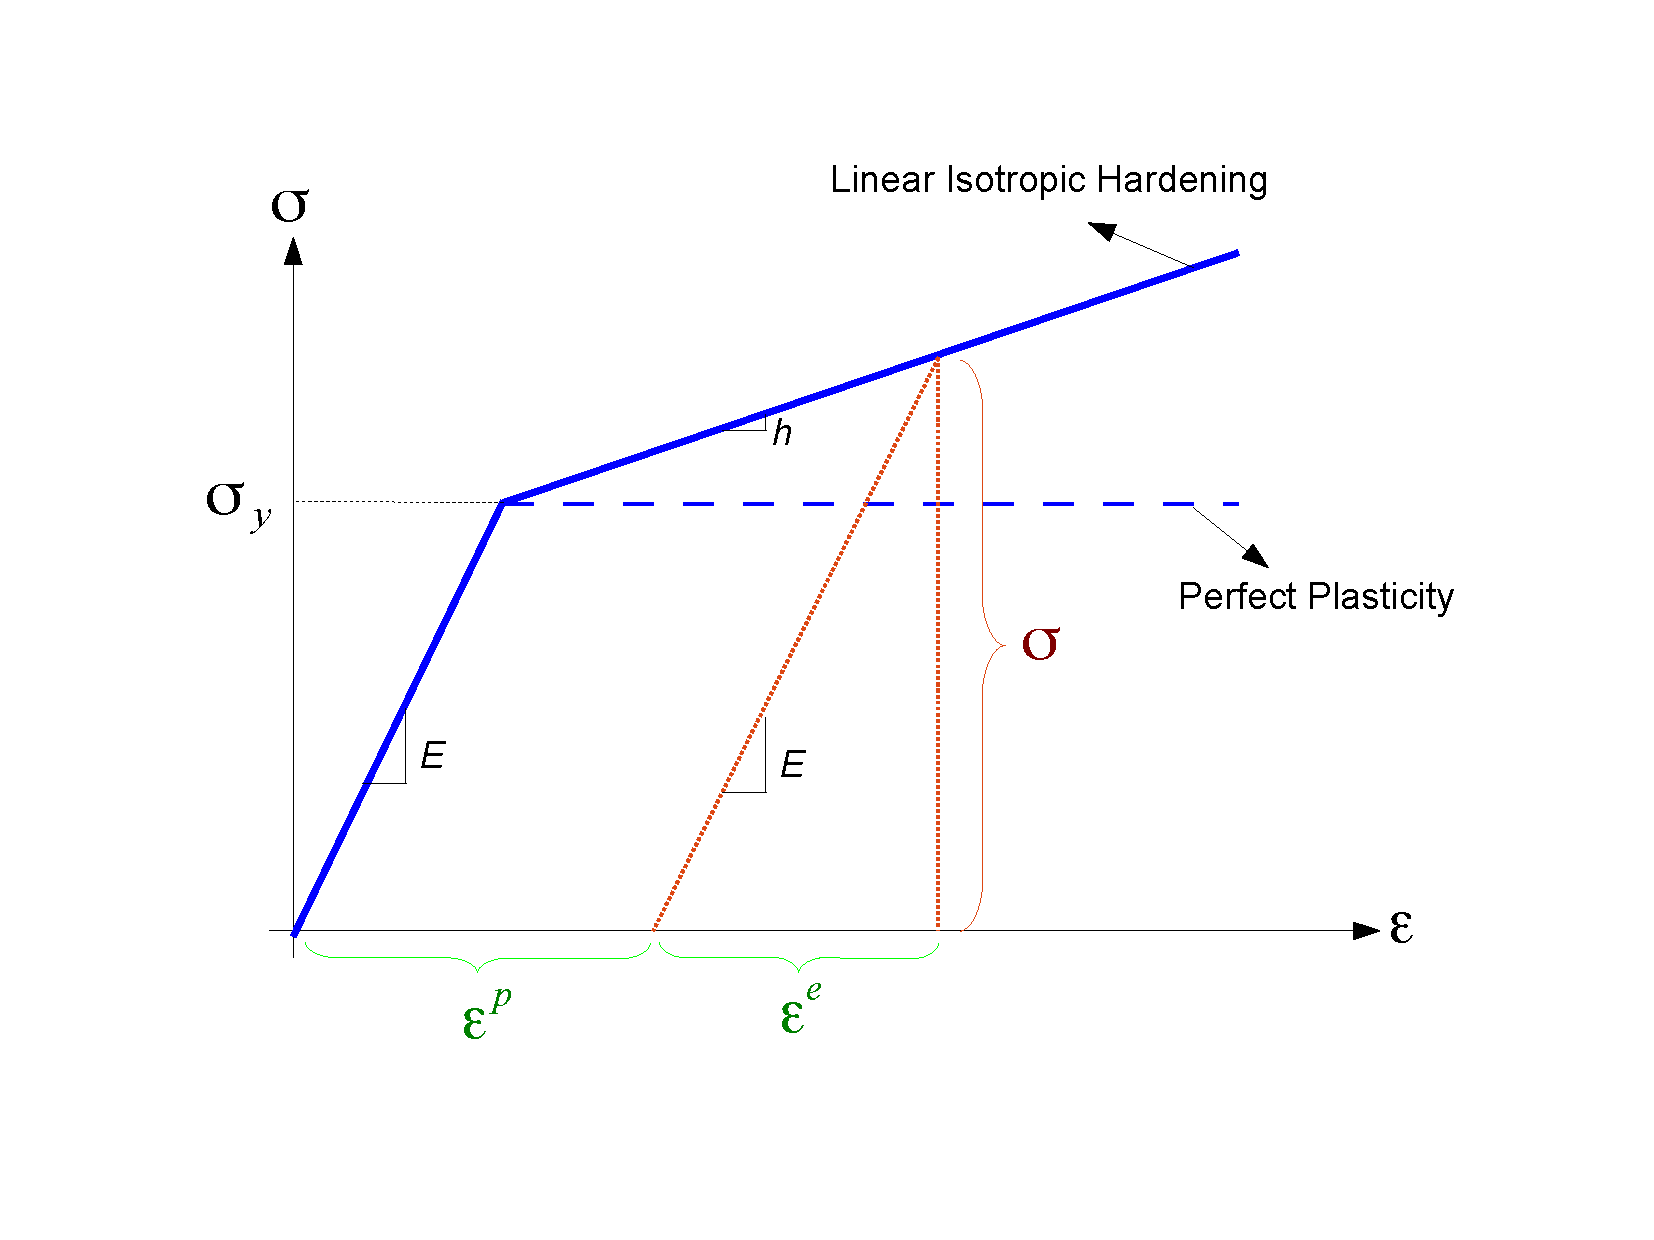
\includegraphics[scale=0.4, clip]{figures/isotropic_hardening_plasticity.pdf}}
   \caption{
    Stress-strain curve for the small-deformation plasticity with linear isotropic hardening.
   }
  \label{fig:smm:cl:Lin-strain-hard}
\end{figure}

\noindent In this class, the von Mises yield criterion is used. In the von Mises yield criterion, the yield is independent of the hydrostatic stress. Other yielding criteria such as Tresca and Gurson can be easily implemented in this class as well.

In the von Mises yield criterion, the hydrostatic stresses have no effect on the plasticity and consequently the yielding occurs when a critical elastic shear energy is achieved.

\begin{equation} \label{eqn:smm:constitutive:von Mises}
	f = \sigma_{\st{eff}} - \sigma_y = (\frac{3}{2} {\mat{\sigma}}^{\st{tr}} : {\mat{\sigma}}^{\st{tr}})^{1/2}-\sigma_y (\mat{\varepsilon}^p)
\end{equation}

\begin{equation} \label{eqn:smm:constitutive:yielding}
 	f < 0 \quad \textrm{Elastic deformation,} \qquad f = 0 \quad  \textrm{Plastic deformation}
\end{equation}

where $\sigma_y$ is the yield strength of the material which can be function of plastic strain in case of hardening type of materials and ${\mat{\sigma}}^{\st{tr}}$ is the deviatoric part of stress given by

\begin{equation} \label{eqn:smm:constitutive:deviatoric stress}
	{\mat{\sigma}}^{\st{tr}}=\mat{\sigma} - \frac{1}{3} trace(\mat{\sigma}) \mat {I}
\end{equation} 

After yielding $(f = 0)$, the normality hypothesis of plasticity determines the direction of plastic flow which is normal to the tangent to the yielding surface at the load point. Then, the tensorial form of the plastic constitutive equation using the von Mises yielding criterion (see equation 4.34) may be written as

\begin{equation} \label{eqn:smm:constitutive:plastic contitutive equation}
	\Delta {\mat{\varepsilon}}^p = \Delta p \frac {\partial{f}}{\partial{\mat \sigma}}=\frac{3}{2} \Delta p \frac{{\mat{\sigma}}^{\st{tr}}}{\sigma_{\st{eff}}}
\end{equation}

In these expressions, the direction of the plastic strain increment (or equivalently, plastic strain rate) is given by $\frac{{\mat{\sigma}}^{\st{tr}}}{\sigma_{\st{eff}}}$ while the magnitude is defined by the plastic multiplier $\Delta p$. This can be obtained using the \emph{consistency condition} which impose the requirement for the load point to remain on the yielding surface in the plastic regime.

\begin{table}[h]
\centering
  \begin{tabular}{| c | l | c |}
    \hline
    1 & Compute the trial stress & ${\mat{\sigma}}^{\st{tr}} = {\mat{\sigma}}_t + 2G\Delta \mat{\varepsilon} + \lambda trace(\Delta \mat{\varepsilon})\mat{I}$ \\[2ex] \hline
    2 & Check the Yielding criteria & $f = (\frac{3}{2} {\mat{\sigma}}^{\st{tr}} : {\mat{\sigma}}^{\st{tr}})^{1/2}-\sigma_y (\mat{\varepsilon}^p)$ \\[2ex] \hline
    3 & Compute the Plastic multiplier & \begin{tabular}{@{}c@{}c@{}} $d \Delta p = \frac{\sigma^{tr}_{eff} - 3G \Delta P^{(k)}- \sigma_y^{(k)}}{3G + h}		
$ \\ $\Delta p^{(k+1)}=\Delta p^{(k)}+ d\Delta p$ \\$\sigma_y^{(k+1)}=(\sigma_y)_t+ h\Delta p$ \end{tabular}\\ [2ex] \hline
    4 & Compute the plastic strain increment & $\Delta {\mat{\varepsilon}}^p = \frac{3}{2} \Delta p \frac{{\mat{\sigma}}^{\st{tr}}}{\sigma_{\st{eff}}}$ \\[2ex] \hline
    5 & Compute the stress increment & ${\Delta \mat{\sigma}} = 2G(\Delta \mat{\varepsilon}-\Delta \mat{\varepsilon}^p) + \lambda  trace(\Delta \mat{\varepsilon}-\Delta \mat{\varepsilon}^p)\mat{I}$ \\[2ex] \hline
    6 & Update the variables & \begin{tabular}{@{}c@{}} ${\mat{\varepsilon^p}}={\mat{\varepsilon}}^p_t+{\Delta {\mat{\varepsilon}}^p}$ \\    ${\mat{\sigma}}={\mat{\sigma}}_t+{\Delta \mat{\sigma}}$ \end{tabular}\\ [2ex] \hline     
    
  \end{tabular}
  \caption{Summary of the implementation procedure of small-deformation plasticity with linear isotropic hardening in \akantu}
  \label{table:equation for small-def plasticity with lin-iso-hardening}
\end{table}


Here, we summarize the implementation procedures for the
small-deformation plasticity with linear isotropic hardening. We use
an implicit integration technique called \emph{the radial return
  method} to obtain the plastic multiplier. This method has the
advantage of being unconditionally stable, however, the accuracy
remains dependent on the step size. The plastic parameters to indicate
in the material file are: \code{$\sigma_y$} (Yield stress) and
\code{h} (Hardening modulus). In addition, the elastic parameters need
to be defined as previously mentioned: \code{E} (Young's modulus),
\code{nu} (Poisson's ratio).


\subsection{Visco-Elasticity}

% Standard Solid rheological model, see [] J.C. Simo, T.J.R. Hughes,
% "Computational Inelasticity", Springer (1998), see Sections 10.2 and 10.3
Visco-elasticity is characterized by strain rate dependent
behavior. Moreover, when such a material undergoes a deformation it
dissipates energy. This dissipation results in a hysteresis loop in
the stress-strain curve at every loading cycle (see
Figure~\ref{fig:smm:cl:visco-elastic:hyst}). In principle, it can be
applied to many materials, since all materials exhibit a visco-elastic
behavior if subjected to particular conditions (such as high
temperatures).
\begin{figure}[!htb]
  \begin{center}

    \subfloat[]{
      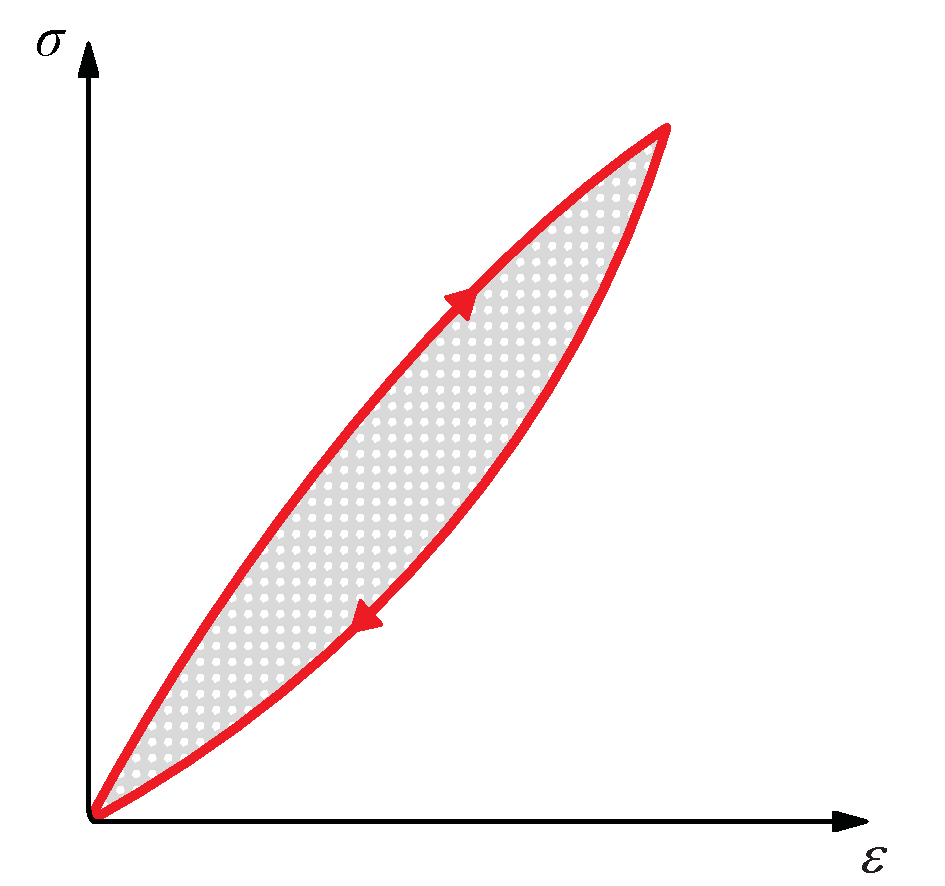
\includegraphics[width=0.4\textwidth,keepaspectratio=true]{figures/stress_strain_visco.pdf}
      \label{fig:smm:cl:visco-elastic:hyst}
    }
    \hspace{0.05\textwidth}
    \subfloat[]{
      \raisebox{0.025\textwidth}{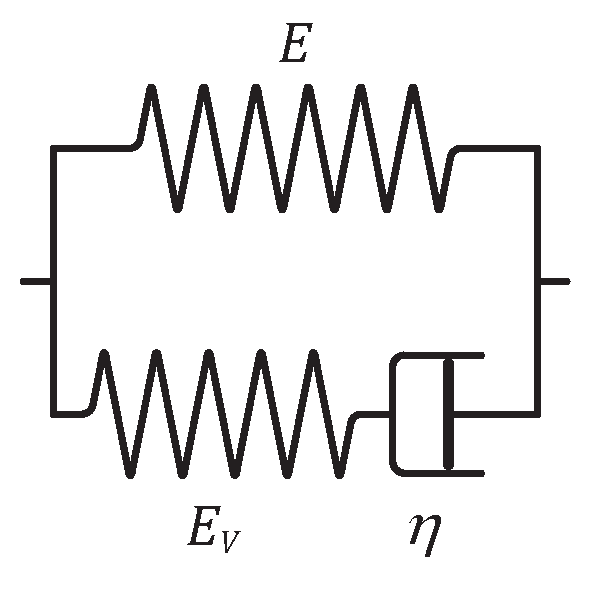
\includegraphics[width=0.3\textwidth,keepaspectratio=true]{figures/visco_elastic_law.pdf}}
      \label{fig:smm:cl:visco-elastic:model}
    }
    \caption{(a) Characteristic stress-strain behavior of a visco-elastic material with hysteresis loop and (b) schematic representation of the standard rheological linear solid visco-elastic model.}
    \label{fig:smm:cl:visco-elastic}
  \end{center}
\end{figure}
The standard rheological linear solid model (see Sections 10.2 and 10.3
of~\cite{simo92}) has been implemented in \akantu. This model results from the
combination of a spring mounted in parallel with a spring and a dashpot
connected in series, as illustrated in
Figure~\ref{fig:smm:cl:visco-elastic:model}. The advantage of this model is that
it allows to account for creep or stress relaxation. The equation that relates
the stress to the strain is (in 1D):
\begin{equation}
  \frac{d\epsilon(t)}{dt} = \left ( E + E_V \right ) ^ {-1} \cdot \left [ \frac{d\sigma(t)}{dt} + \frac{E_V}{\eta}\sigma(t) - \frac{EE_V}{\eta}\epsilon(t) \right ]
\end{equation}
where $\eta$ is the viscosity. The equilibrium condition is unique and
is attained in the limit, as $t \to \infty $. At this stage, the
response is elastic and depends on the Young's modulus $E$.  The
mandatory parameters for the material file are the following:
\code{rho} (density), \code{E} (Young's modulus), \code{nu} (Poisson's
ratio), \code{Plane\_Stress} (if set to zero plane strain, otherwise
plane stress), \code{eta} (dashpot viscosity) and \code{Ev} (stiffness
of the viscous element).

Note that the current standard linear solid model is applied only on the deviatoric part of the strain tensor. The spheric part of the strain tensor affects the stress tensor like an linear elastic material.

\subsection{Damage}

In the  simplified case of a  linear elastic and brittle  material, isotropic
damage can be represented by a scalar variable $d$, which varies from $0$ to $1$
for  no  damage  to  fully  broken  material  respectively.  The  stress-strain
relationship then becomes:
\begin{equation*}
  \mat{\sigma} = (1-d)\, \mat{C}:\mat{\varepsilon}
\end{equation*}

where  $\mat{\sigma}$,  $\mat{\varepsilon}$ are  the  Cauchy  stress and  strain
tensors, and $\mat{C}$ is the elastic stiffness tensor. This formulation relies
on the definition of an evolution law for the damage variable. In \akantu, many
possibilities exist and they are listed below.

\subsubsection{Marigo}
This damage evolution law is energy based as defined by Marigo \cite{marigo81a,
  lemaitre96a}. It is an isotropic damage law.
\begin{align}
  Y &= \frac{1}{2}\mat{\varepsilon}:\mat{C}:\mat{\varepsilon}\\
  F &= Y - Y_d - S d\\
  d &= \left\{
    \begin{array}{l l}
      \mathrm{min}\left(\frac{Y-Y_d}{S},\;1\right) & \mathrm{if}\; F > 0\\
      \mathrm{unchanged} & \mathrm{otherwise}
    \end{array}
  \right.
\end{align}
In this formulation, $Y$ is the strain energy release rate, $Y_d$ the
rupture criterion and $S$ the damage energy.  The non-local version of
this damage evolution law is constructed by averaging the energy $Y$.

\subsubsection{Mazars}
This law introduced by Mazars \cite{mazars84a} is a behavioral model to
represent damage evolution in concrete. The governing variable in this damage
law is the equivalent strain $\varepsilon_{\st{eq}} =
\sqrt{<\mat{\varepsilon}>_+:<\mat{\varepsilon}>_+}$, with $<.>_+$ the positive
part of the tensor.
The damage the is defined as:
\begin{align}
  D &= \alpha_t^\beta D_t + (1-\alpha_t)^\beta D_c\\
  D_t &= 1 - \frac{\kappa_0 (1- A_t)}{\varepsilon_{\st{eq}}} - A_t \exp^{-B_t(\varepsilon_{\st{eq}}-\kappa_0)}\\
  D_c &= 1 - \frac{\kappa_0 (1- A_c)}{\varepsilon_{\st{eq}}} - A_c
  \exp^{-B_c(\varepsilon_{\st{eq}}-\kappa_0)}\\
  \alpha_t &= \frac{\sum_{i=1}^3<\varepsilon_i>_+\varepsilon_{\st{nd}\;i}}{\varepsilon_{\st{eq}}^2}
\end{align}
With $\kappa_0$ the damage threshold, $A_t$ and $B_t$ the damage parameter in
traction, $A_c$ and $B_c$ the damage parameter in compression, $\beta$ is the
shear parameter. $\alpha_t$ is the coupling parameter between traction and
compression, the $\varepsilon_i$ are the eigenstrain and the
$\varepsilon_{\st{nd}\;i}$ are the eigenvalues of the strain if the material
were undamaged.

The coefficients $A$ and $B$ are the post-peak asymptotic
value and the decay shape parameters.


\subsection{Summary}\index{Material!List}

The list of all the materials available in Akantu is summarized in Tables \ref{tab:smm:cl:summary:list} as well as the keyword required for each material and the assosiated material properties.

\begin{table}[h!]
  \begin{center}
\begin{tabular}[c]{ m{3.5cm} | l | c | p{3.5cm} }
Material & Keyword & Parameter & Description \\
\hline
%%%%%%%%%%%%%%%%%
Linear elastic isotropic & \code{elastic} & -  & Table \ref{tab:smm:cl:summary:base}\\
\hline
%%%%%%%%%%%%%%%%%%
Linear elastic orthotropic  & \code{elastic\_orthotropic} & \code{Cij} & Tangent matrix coefficients (i,j = 1,2, ... voigt size ) \\
\hline
%%%%%%%%%%%%%%%%%%
Linear elastic anisotropic  & \code{elastic\_anisotropic} & \code{n1} & Direction of main material axis \\
 & & \code{n2} & Direction of secondary material axis \\
 & & \code{n3} & Direction of tertiery material axis \\
 & & \code{Cij} & Tangent matrix coefficients (i,j = 1,2, ... voigt size ) \\
 & & \code{alpha} & Proportion of viscous stress\\
\hline
%%%%%%%%%%%%%%%%%%
Neohookean (Finite-strain) \cite{Belytschko:2000} & \code{neohookean} & -  & Table \ref{tab:smm:cl:summary:base}\\
\hline
%%%%%%%%%%%%%%%%%%
Standard linear solid \cite{simo92} & \multirow{2}{*}{\code{sls\_deviatoric}} & - & Table \ref{tab:smm:cl:summary:base}\\
 & &  \code{Eta} & Viscosity\\
 & & \code{Ev} & Stiffness of the viscous element \\
\hline
%%%%%%%%%%%%%%%%%%
Elasto-plastic linear isotropic hardening & \code{plastic\_linear\_isotropic\_hardening}  & - & Table \ref{tab:smm:cl:summary:base}\\
 & &  \code{h} & Hardening modulus\\
 & &  \code{sigma\_y} & Yielding stress\\
\hline
%%%%%%%%%%%%%%%%%%
Visco-plastic & \code{visco\_plastic}  & - & Table \ref{tab:smm:cl:summary:base}\\
 & &  \code{rate} & Rate sensitivity component\\
 & &  \code{edot0} & Reference strain rate\\
 & &  \code{ts} & Time \\
\hline
\end{tabular}
\end{center}
  \caption{List of material properties with their corresponding keywords and material parameters.}
  \label{tab:smm:cl:summary:list}
\end{table}

\vspace{0.5cm}

In addition to the properties presented in Table \ref{tab:smm:cl:summary:list}, every material also has the parameter ''\code{rho}`` which corresponds to the density. The properties listed in Table  \ref{tab:smm:cl:summary:base} correspond to the parameters required to describe a linear elastic isotropic material, however those parameters are also commun to most of the materials available as previously described in Table \ref{tab:smm:cl:summary:list}.

\begin{table}[h!]
  \begin{center}
\begin{tabular}[c]{  l | p{6.5cm} }\label{tab:smm:cl:summary:base}
Parameter & Description \\
\hline
%%%%%%%%%%%%%%%%%
\code{rho}  & Density\\
\code{E}  & Young's modulus\\
\code{nu}  & Poisson's ratio\\
\code{Plane\_Stress} & Plane stress simplification (only 2D problems)\\
\hline
\end{tabular}
\end{center}
  \caption{List of material parameters shared my most materials}
  \label{tab:smm:cl:summary:base}
\end{table}

%%% Local Variables:
%%% mode: latex
%%% TeX-master: "manual"
%%% End:
}{}

\IfFileExists{manual-cohesive_laws.tex}{\subsection{Cohesive laws}
\label{sec:cohesive-laws}

\subsubsection{Linear Irreversible Law\matlabel{ssect:smm:cl:coh-snozzi}}

\begin{figure}[!hbt]
  \centering
  \subfloat[Linear]{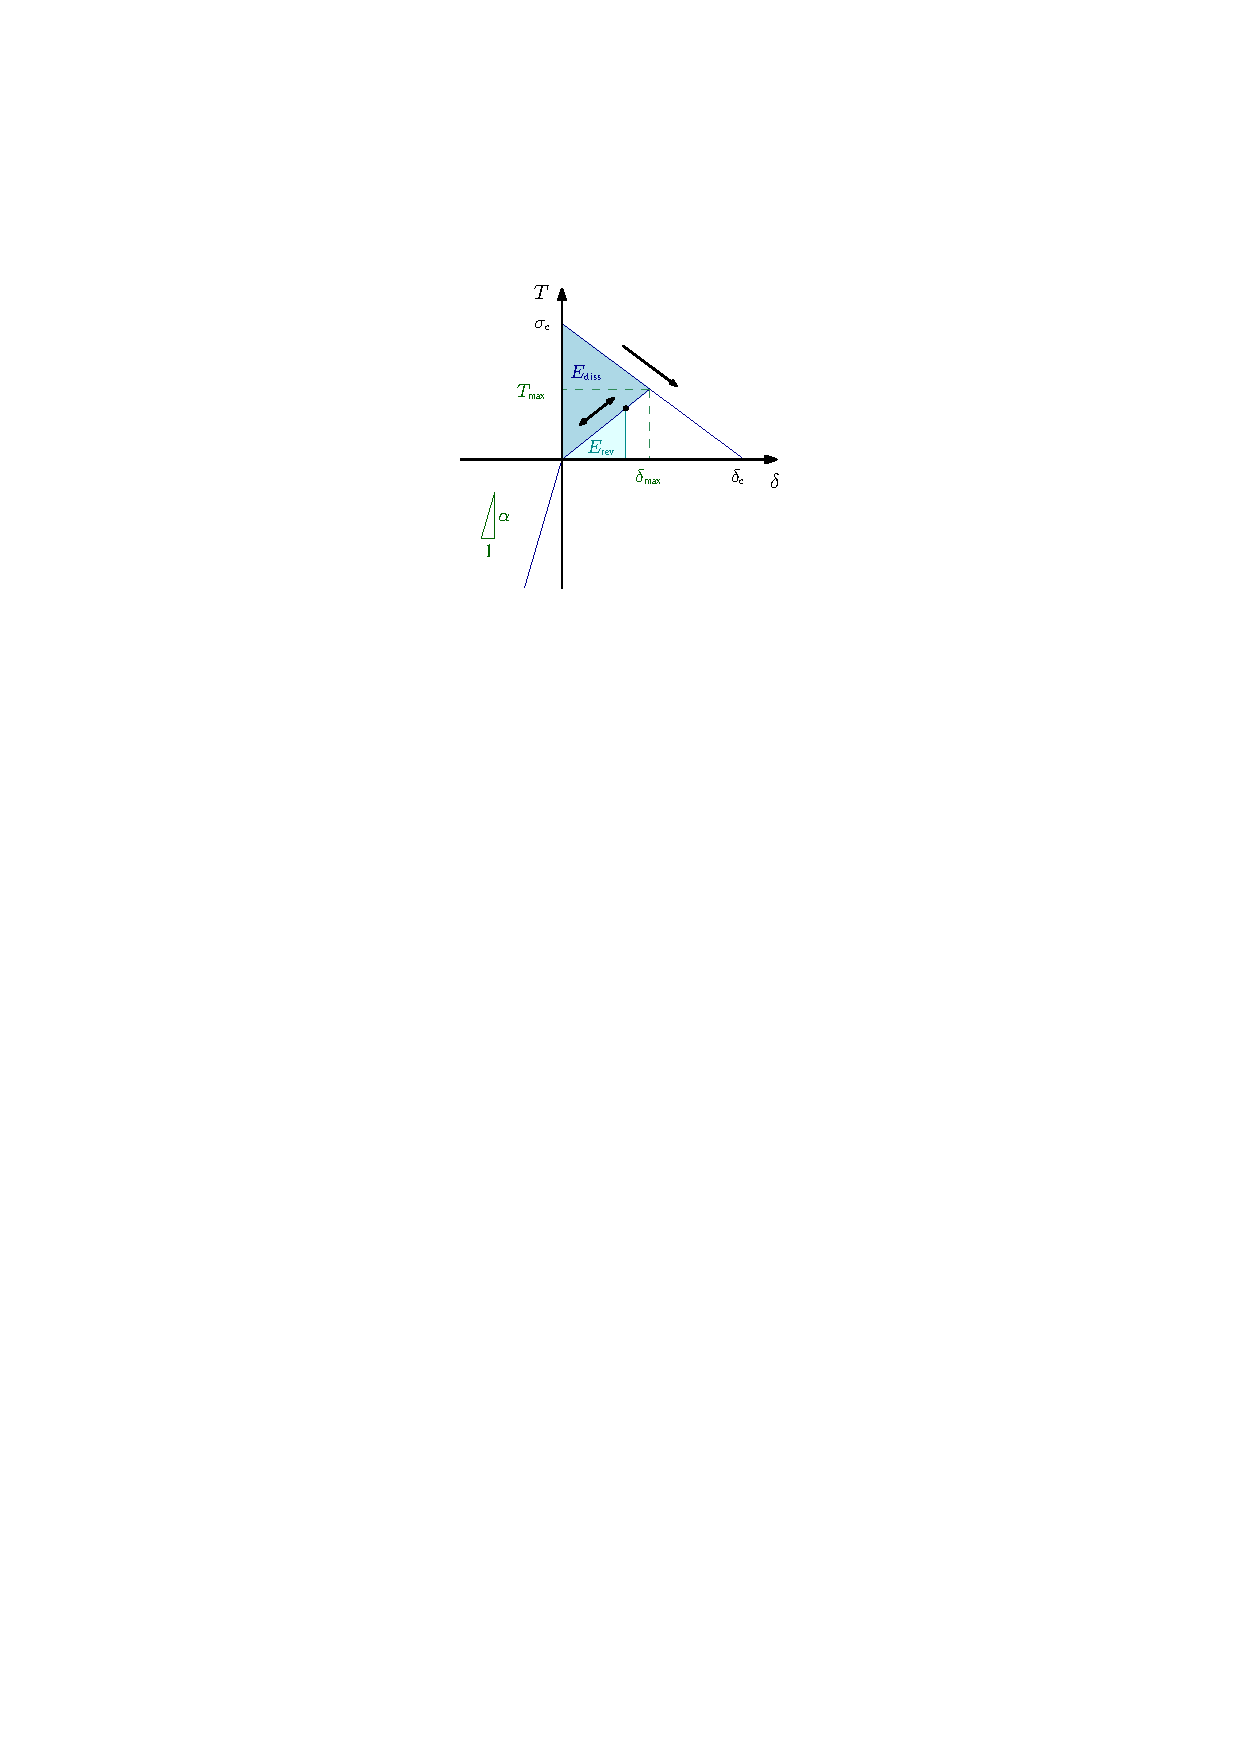
\includegraphics[width=0.4\textwidth]{figures/linear_cohesive_law}}
  \qquad
  \subfloat[Bilinear]{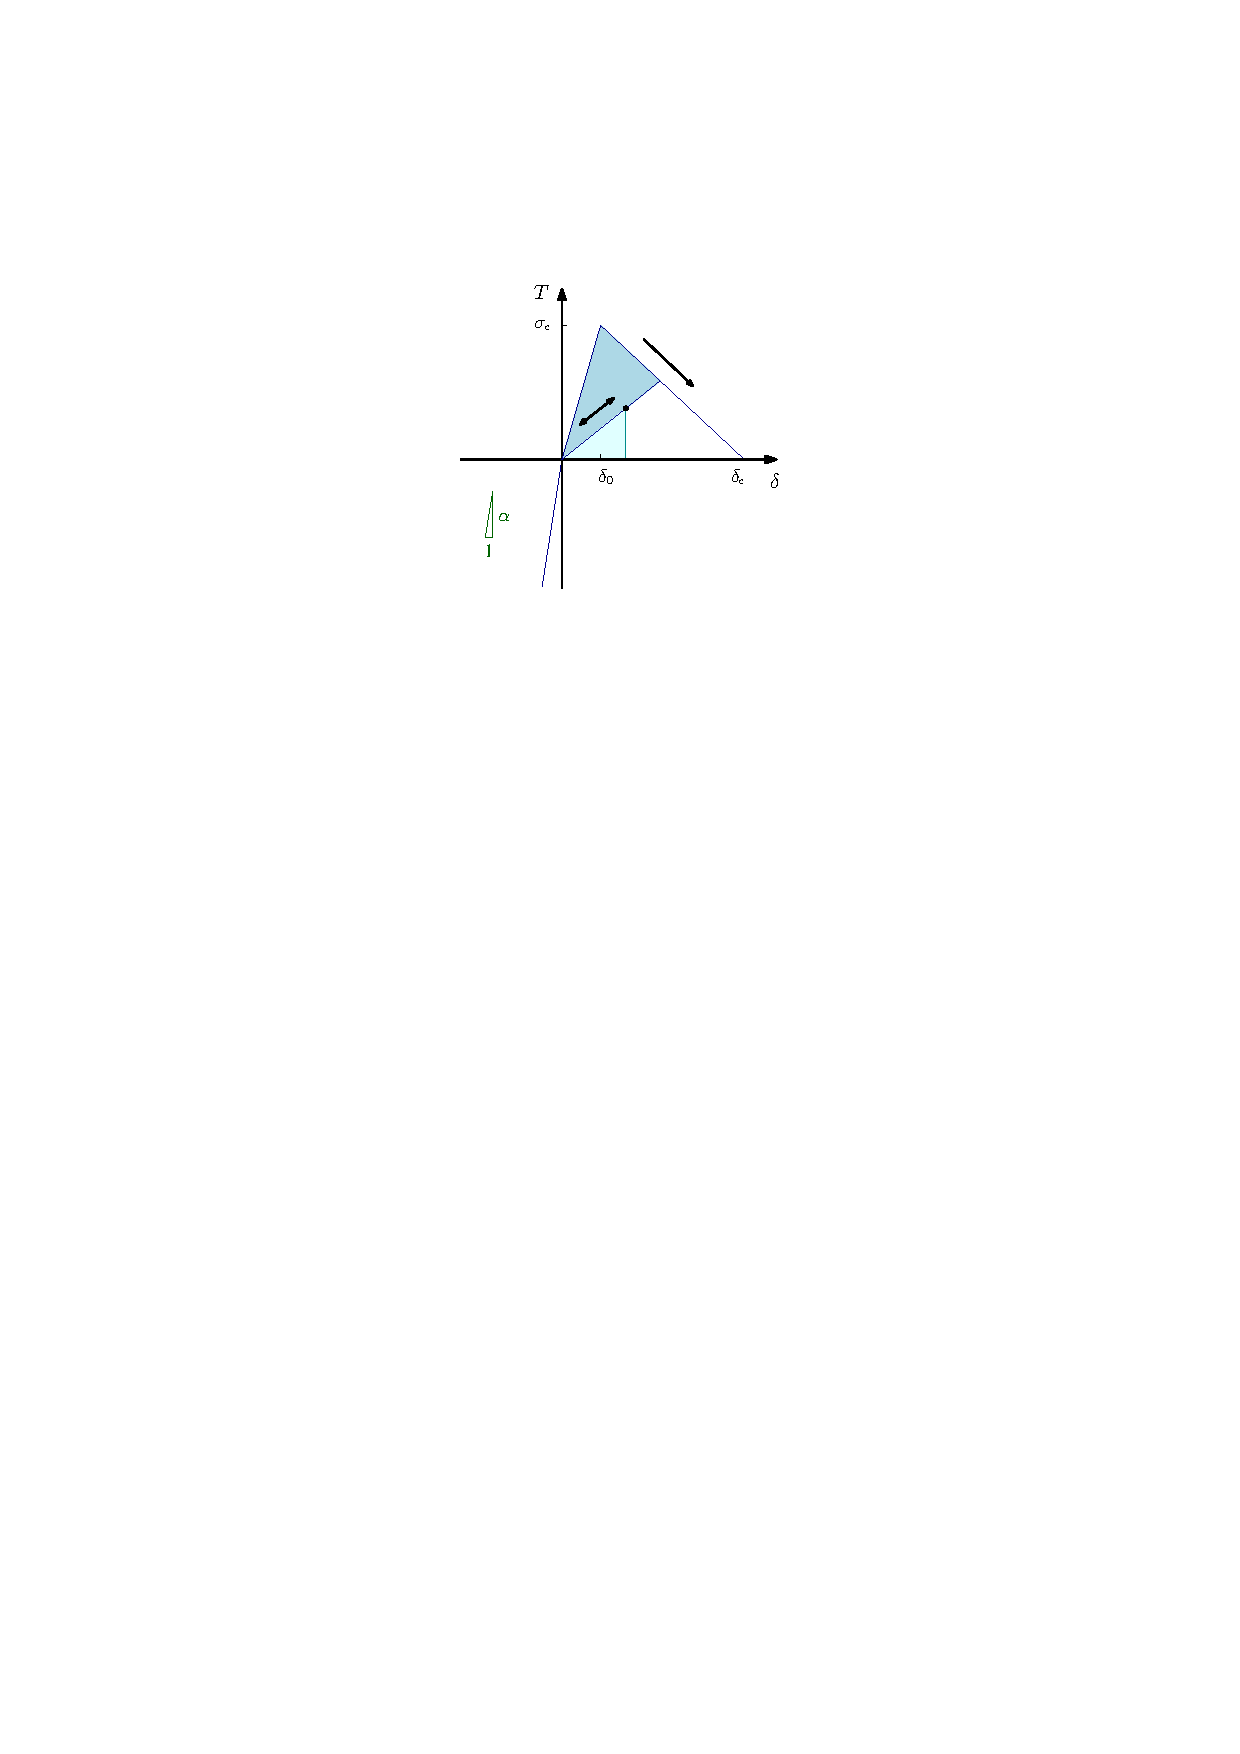
\includegraphics[width=0.4\textwidth]{figures/bilinear_cohesive_law}}
  \caption{Irreversible cohesive laws for explicit simulations.}
  \label{fig:smm:coh:linear_cohesive_law}
\end{figure}

\akantu includes the Snozzi-Molinari~\cite{snozzi_cohesive_2013}
linear irreversible cohesive law (see
Figure~\ref{fig:smm:coh:linear_cohesive_law}). It is an extension to
the Camacho-Ortiz~\cite{camacho_computational_1996} cohesive law in
order to make dissipated fracture energy path-dependent. The concept
of free potential energy is dropped and a new independent parameter
$\kappa$ is introduced:
\begin{equation}
  \kappa = \frac{G_\mathrm{c, II}}{G_\mathrm{c, I}}
\end{equation}

where $G_\mathrm{c, I}$ and $G_\mathrm{c, II}$ are the
necessary works of separation per unit area to open completely a
cohesive zone under mode I and mode II, respectively. Their model yields to the
following equation for cohesive tractions $\vec{T}$ in case of crack
opening ${\delta}$:
\begin{equation}
  \label{eq:smm:coh:tractions}
  \vec{T} = \left( \frac{\beta^2}{\kappa} \Delta_\mathrm{t} \vec{t} +
    \Delta_\mathrm{n} \vec{n} \right)
  \frac{\sigma_\mathrm{c}}{\delta}
  \left( 1- \frac{\delta}{\delta_\mathrm{c}} \right)
  = \hat{\vec T}\,
  \frac{\sigma_\mathrm{c}}{\delta}
  \left( 1- \frac{\delta}{\delta_\mathrm{c}} \right)
\end{equation}

where $\sigma_\mathrm{c}$ is the material strength along the fracture,
$\delta_\mathrm{c}$ the critical effective displacement after which
cohesive tractions are zero (complete decohesion), $\Delta_\mathrm{t}$
and $\Delta_\mathrm{n}$ are the tangential and normal components of
the opening displacement vector $\vec{\Delta}$, respectively. The
parameter $\beta$ is a weight that indicates how big the tangential
opening contribution is. The effective opening displacement is:
\begin{equation}
  \delta = \sqrt{\frac{\beta^2}{\kappa^2} \Delta_\mathrm{t}^2 +
    \Delta_\mathrm{n}^2}
\end{equation}
In case of unloading or reloading $\delta < \delta_\mathrm{max}$,
tractions are calculated as:
\begin{align}
  T_\mathrm{n} &= \Delta_\mathrm{n}\,
  \frac{\sigma_\mathrm{c}}{\delta_\mathrm{max}}
  \left( 1- \frac{\delta_\mathrm{max}}{\delta_\mathrm{c}} \right) \\
  T_\mathrm{t} &= \frac{\beta^2}{\kappa}\, \Delta_\mathrm{t}\,
  \frac{\sigma_\mathrm{c}}{\delta_\mathrm{max}}
  \left( 1- \frac{\delta_\mathrm{max}}{\delta_\mathrm{c}} \right)
\end{align}
so that they vary linearly between the origin and the maximum attained
tractions. As shown in Figure~\ref{fig:smm:coh:linear_cohesive_law},
in this law, the dissipated and reversible energies are:
\begin{align}
  E_\mathrm{diss} &= \frac{1}{2} \sigma_\mathrm{c}\, \delta_\mathrm{max}\\[1ex]
  E_\mathrm{rev} &= \frac{1}{2} T\, \delta
\end{align}
Moreover, a damage parameter $D$ can be defined as:
\begin{equation}
  D = \min \left(
    \frac{\delta_\mathrm{max}}{\delta_\mathrm{c}},1 \right)
\end{equation}
which varies from 0 (undamaged condition) and 1 (fully
damaged condition). This variable can only increase because damage is
an irreversible process. A simple penalty contact model has been incorporated
in the cohesive law so that normal tractions can be returned in
case of compression:
\begin{equation}
  T_\mathrm{n} = \alpha \Delta_\mathrm{n} \quad\text{if
    $\Delta_\mathrm{n} < 0$}
\end{equation}
where $\alpha$ is a stiffness parameter that defaults to zero. The
relative contact energy is equivalent to reversible energy but in
compression.

The material name of the linear decreasing cohesive law  is
\code{material\_cohesive\_linear} and its parameters with their
respective default values are:
\begin{itemize}
\item \code{sigma\_c}: 0
\item \code{delta\_c}: 0
\item \code{beta}: 0
\item \code{G\_c}: 0
\item \code{kappa}: 1
\item \code{penalty}: 0
\end{itemize}
where \code{G\_c} corresponds to $G_\mathrm{c, I}$. A random number
generator can be used to assign a random $\sigma_\mathrm{c}$ to each
facet following a given distribution (see
Section~\ref{sect:smm:CL}). Only one parameter between \code{delta\_c}
and \code{G\_c} has to be specified. For random $\sigma_\mathrm{c}$
distributions, the chosen parameter of these two is kept fixed and the
other one is varied.

The bilinear constitutive law works exactly the same way as the linear
one, except for the additional parameter \code{delta\_0} that by
default is zero. Two examples for the extrinsic and intrinsic cohesive
elements and also an example to assign different properties to
intergranular and transgranular cohesive elements can be found in
the folder \code{\examplesdir/cohesive\_element/}.

\subsubsection{Linear Cohesive Law with Fatigue\matlabel{ssect:smm:cl:coh-fatigue}}

This law represents a variation of the linear irreversible cohesive
law of the previous section, that removes the hypothesis of elastic
unloading-reloading cycles. With this law, some energy is dissipated
also during unloading and reloading with hysteresis. The
implementation follows the work of~\cite{nguyen2001}. During the
unloading-reloading cycle, the traction increment is computed as
\begin{equation}
  \dot{T} =
  \begin{cases}
    K^- \, \dot{\delta} & \text{if $\dot{\delta} < 0$} \\
    K^+ \, \dot{\delta} & \text{if $\dot{\delta} > 0$} \\
  \end{cases}
\end{equation}
where $\dot{\delta}$ and $\dot{T}$ are respectively the effective
opening displacement and the cohesive traction increments with respect
to time, while $K^-$ and $K^+$ are respectively the unloading and
reloading incremental stiffness. The unloading path is linear and
results in an unloading stiffness
\begin{equation}
  K^- = \frac{T_\mathrm{max}}{\delta_\mathrm{max}}
\end{equation}
where $T_\mathrm{max}$ and $\delta_\mathrm{max}$ are the maximum
cohesive traction and the effective opening displacement reached
during the precedent loading phase. The unloading stiffness remains
constant during the unloading phase. On the other hand the reloading
stiffness increment $\dot{K}^+$ is calculated as
\begin{equation}
  \dot{K}^+ =
  \begin{cases}
    - K^+ \, \dot{\delta} / \delta_\mathrm{f} & \text{if $\dot{\delta}
      > 0$} \\
    \left( K^+ - K^- \right) \, \dot{\delta} / \delta_\mathrm{f} &
    \text{if $\dot{\delta} < 0$}
  \end{cases}
\end{equation}
where $\delta_\mathrm{f}$ is a material parameter. During unloading
the stiffness $K^+$ tends to $K^-$, while during reloading $K^+$ gets
decreased at every time step. If the cohesive traction during
reloading exceeds the upper limit given by
equation~\eqref{eq:smm:coh:tractions}, it is recomputed following the
behavior of the linear decreasing cohesive law for crack opening.

\subsubsection{Exponential Cohesive Law\matlabel{ssect:smm:cl:coh-exponential}}

Ortiz and Pandolfi proposed this cohesive law in 1999~\cite{ortiz1999}.  The
traction-opening equation for this law is as follows:
\begin{equation}
  \label{eq:exponential_law}
  T = e \sigma_c \frac{\delta}{\delta_c}e^{-\delta/ \delta_c}
\end{equation}
This equation is plotted in Figure~\ref{fig:smm:CL:ECL}. The term
$\partial{\vec{T}}/ \partial{\delta}$ of
equation~\eqref{eq:cohesive_stiffness} after the necessary derivation
can expressed as
\begin{equation}
  \label{eq:tangent_cohesive}
  \frac{\partial{\vec{T}}} {\partial{\delta}} = \hat{\vec{T}} \otimes
  \frac                       {\partial{(T/\delta)}}{\partial{\delta}}
  \frac{\hat{\vec{T}}}{\delta}+ \frac{T}{\delta}  \left[ \beta^2 \mat{I} +
  \left(1-\beta^2\right) \left(\vec{n} \otimes \vec{n}\right)\right]
\end{equation}
where
\begin{equation}
  \frac{\partial{(T/ \delta)}}{\partial{\delta}} = \left\{\begin{array} {l l}
      -e  \frac{\sigma_c}{\delta_c^2  }e^{-\delta  /  \delta_c} &  \quad  if
      \delta \geq \delta_{max}\\
      0 & \quad if \delta < \delta_{max}, \delta_n > 0
    \end{array} \right.
\end{equation}


\begin{figure}[!htb]
  \begin{center}
    \includegraphics[width=0.6\textwidth,keepaspectratio=true]{figures/cohesive_exponential.pdf}
    \caption{Exponential cohesive law}
    \label{fig:smm:CL:ECL}
  \end{center}
\end{figure}


%%% Local Variables:
%%% mode: latex
%%% TeX-master: "manual"
%%% End:
}{}


%%% Local Variables:
%%% mode: latex
%%% TeX-master: "manual"
%%% End:


\section{Adding a New Constitutive Law}\index{Material!create a new
material}

There are several constitutive laws in \akantu as described in the
previous Section~\ref{sect:smm:CL}. It is also possible to use a
user-defined material for the simulation. These materials are referred
to as local materials since they are local to the example of the user
and not part of the \akantu library.  To define a new local material,
two files (\code {material\_XXX.hh} and \code{material\_XXX.cc}) have
to be provided where \code{XXX} is the name of the new material. The
header file \code {material\_XXX.hh} defines the interface of your
custom material. Its implementation is provided in the
\code{material\_XXX.cc}. The new law must inherit from the
\code{Material} class or any other existing material class. It is
therefore necessary to include the interface of the parent material
in the header file of your local material and indicate the inheritance
in the declaration of the class:
\begin{cpp}
/* ---------------------------------------------------------------------- */
#include "material.hh"
/* ---------------------------------------------------------------------- */

#ifndef __AKANTU_MATERIAL_XXX_HH__
#define __AKANTU_MATERIAL_XXX_HH__

namespace akantu {

class MaterialXXX : public Material {

/// declare here the interface of your material

};
\end{cpp}
In the header file the user also needs to declare all the members of the new
material. These include the parameters that a read from the
material input file, as well as any other material parameters that will be
computed during the simulation and internal variables.


In the following the example of adding a new damage material will be
presented. In this case the parameters in the material will consist of the
Young's modulus, the Poisson coefficient, the resistance to damage and the
damage threshold. The material will then from these values compute its Lam\'{e}
coefficients and its bulk modulus. Furthermore, the user has to add a new
internal variable \code{damage} in order to store the amount of damage at each
quadrature point in each step of the simulation. For this specific material the
member declaration inside the class will look as follows:
\begin{cpp}
class LocalMaterialDamage : public Material {

/// declare constructors/destructors here

/// declare methods and accessors here

  /* -------------------------------------------------------------------- */
  /* Class Members                                                        */
  /* -------------------------------------------------------------------- */

  AKANTU_GET_MACRO_BY_ELEMENT_TYPE_CONST(Damage, damage, Real);
private:

  /// the young modulus
  Real E;

  /// Poisson coefficient
  Real nu;

  /// First Lame coefficient
  Real lambda;

  /// Second Lame coefficient (shear modulus)
  Real mu;

  /// resistance to damage
  Real Yd;

  /// damage threshold
  Real Sd;

  /// Bulk modulus
  Real kpa;

  /// damage internal variable
  InternalField<Real> damage;

};
\end{cpp}
In order to enable to print the material parameters at any point in
the user's example file using the standard output stream by typing:
\begin{cpp}
for (UInt m = 0; m  < model.getNbMaterials(); ++m)
  std::cout << model.getMaterial(m) << std::endl;
\end{cpp}
the standard output stream operator has to be redefined. This should be done at the end of the header file:
\begin{cpp}
class LocalMaterialDamage : public Material {

  /// declare here the interace of your material

}:
/* ---------------------------------------------------------------------- */
/* inline functions                                                       */
/* ---------------------------------------------------------------------- */
/// standard output stream operator
inline std::ostream & operator <<(std::ostream & stream, const LocalMaterialDamage & _this)
{
  _this.printself(stream);
  return stream;
}
\end{cpp}
However, the user still needs to register the material parameters that
should be printed out. The registration is done during the call of the
constructor. Like all definitions the implementation of the
constructor has to be written in the \code{material\_XXX.cc}
file. However, the declaration has to be provided in the
\code{material\_XXX.hh} file:
\begin{cpp}
class LocalMaterialDamage : public Material {
  /* -------------------------------------------------------------------- */
  /* Constructors/Destructors                                             */
  /* -------------------------------------------------------------------- */
public:

  LocalMaterialDamage(SolidMechanicsModel & model, const ID & id = "");
};
\end{cpp}
The user can now define the implementation of the constructor in the
\code{material\_XXX.cc} file:
\begin{cpp}
/* ---------------------------------------------------------------------- */
#include "local_material_damage.hh"
#include "solid_mechanics_model.hh"

namespace akantu {

/* ---------------------------------------------------------------------- */
LocalMaterialDamage::LocalMaterialDamage(SolidMechanicsModel & model,
					 const ID & id)  :
  Material(model, id),
  damage("damage", *this) {
  AKANTU_DEBUG_IN();

  this->registerParam("E", E, 0., _pat_parsable, "Young's modulus");
  this->registerParam("nu", nu, 0.5, _pat_parsable, "Poisson's ratio");
  this->registerParam("lambda", lambda, _pat_readable, "First Lame coefficient");
  this->registerParam("mu", mu, _pat_readable, "Second Lame coefficient");
  this->registerParam("kapa", kpa, _pat_readable, "Bulk coefficient");
  this->registerParam("Yd", Yd,   50., _pat_parsmod);
  this->registerParam("Sd", Sd, 5000., _pat_parsmod);

  damage.initialize(1);

  AKANTU_DEBUG_OUT();
}
\end{cpp}
During the intializer list the reference to the model and the material id are
assigned and the constructor of the internal field is called. Inside the scope
of the constructor the internal values have to be initialized and the
parameters, that should be printed out, are registered with the function:
\code{registerParam}\index{Material!registerParam}:
\begin{cpp}
void registerParam(name of the parameter (key in the material file),
		   member variable,
		   default value (optional parameter),
		   access permissions,
		   description);
\end{cpp}
The available access permissions are as follows:
\begin{itemize}
  \item \code{\_pat\_internal}: Parameter can only be output when the material is printed.
  \item \code{\_pat\_writable}: User can write into the parameter. The parameter is output when the material is printed.
  \item \code{\_pat\_readable}: User can read the parameter. The parameter is output when the material is printed.
  \item \code{\_pat\_modifiable}: Parameter is writable and readable.
  \item \code{\_pat\_parsable}: Parameter can be parsed, \textit{i.e.} read from the input file.
  \item \code{\_pat\_parsmod}: Parameter is modifiable and parsable.
\end{itemize}

In order to implement the new constitutive law the user needs to
specify how the additional material parameters, that are not
defined in the input material file, should be calculated. Furthermore,
it has to be defined how stresses and the stable time step should be
computed for the new local material. In the case of implicit
simulations, in addition, the computation of the tangent stiffness needs
to be defined. Therefore, the user needs to redefine the following
functions of the parent material:
\begin{cpp}
void initMaterial();

// for explicit and implicit simulations void
computeStress(ElementType el_type, GhostType ghost_type = _not_ghost);

// for implicit simulations
void computeTangentStiffness(const ElementType & el_type,
			     Array<Real> & tangent_matrix,
			     GhostType ghost_type = _not_ghost);

// for explicit and implicit simulations
Real getStableTimeStep(Real h, const Element & element);
\end{cpp}
In the following a detailed description of these functions is provided:
\begin{itemize}

\item \code{initMaterial}:~ This method is called after the material
  file is fully read and the elements corresponding to each material
  are assigned. Some of the frequently used constant parameters are
  calculated in this method. For example, the Lam\'{e} constants of
  elastic materials can be considered as such parameters.

\item \code{computeStress}:~ In this method, the stresses are
  computed based on the constitutive law as a function of the  strains of the
  quadrature points.  For example, the stresses for the elastic
  material are calculated based on the following formula:
  \begin{equation}
    \label{eqn:smm:constitutive_elastic}
    \mat{\sigma }  =\lambda\mathrm{tr}(\mat{\varepsilon})\mat{I}+2 \mu \mat{\varepsilon}
  \end{equation}

  Therefore, this method contains a loop on all quadrature points
  assigned to the material using the two macros:\par
  \code{MATERIAL\_STRESS\_QUADRATURE\_POINT\_LOOP\_BEGIN}\par
  \code{MATERIAL\_STRESS\_QUADRATURE\_POINT\_LOOP\_END}

  \begin{cpp}
    MATERIAL_STRESS_QUADRATURE_POINT_LOOP_BEGIN(element_type);

    // sigma <- f(grad_u)

    MATERIAL_STRESS_QUADRATURE_POINT_LOOP_END;
  \end{cpp}

  \note{The strain vector in \akantu contains the values of $\nabla
\vec{u}$, i.e. it is really the \emph{displacement gradient},}

\item \code{computeTangentStiffness}:~ This method is called when
  the tangent to the stress-strain curve is desired (see Fig \ref
  {fig:smm:AL:K}).  For example, it is called in the implicit solver
  when the stiffness matrix for the regular elements is assembled
  based on the following formula:
  \begin{equation}
    \label{eqn:smm:constitutive_elasc} \mat{K }
    =\int{\mat{B^T}\mat{D(\varepsilon)}\mat{B}}
  \end{equation}

  Therefore, in this method, the \code{tangent} matrix (\mat{D}) is
  computed for a given strain.

  \note{ The \code{tangent} matrix is a $4^{th}$ order tensor which is
    stored as a matrix in Voigt notation.}

  \begin{figure}[!htb]
    \begin{center}
      \includegraphics[width=0.4\textwidth,keepaspectratio=true]{figures/tangent.pdf}
      \caption{Tangent to the stress-strain curve.}
      \label{fig:smm:AL:K}
    \end{center}
  \end{figure}

\item \code{getCelerity}:~The stability criterion of the explicit integration scheme depend on the fastest wave celerity~\eqref{eqn:smm:explicit:stabletime}. This celerity depend on the material, and therefore the value of this velocity should be defined in this method for each new material. By default, the fastest wave speed is the compressive wave whose celerity can be defined in~\code{getPushWaveSpeed}.
\end{itemize}
Once the declaration and implementation of the new material has been
completed, this material can be used in the user's example by including the header file:
\begin{cpp}
#include "material_XXX.hh"
\end{cpp}
For existing materials, as mentioned in Section~\ref{sect:smm:CL}, by
default, the materials are initialized inside the method
\code{initFull}. If a local material should be used instead, the
initialization of the material has to be postponed until the local
material is registered in the model. Therefore, the model is
initialized with the boolean for skipping the material initialization
equal to true:
\begin{cpp}
/// model initialization
model.initFull(_analysis_method = _explicit_lumped_mass);
\end{cpp}
Once the model has been initialized, the local material needs
to be registered in the model:
\begin{cpp}
model.registerNewCustomMaterials<XXX>("name_of_local_material");
\end{cpp}
Only at this point the material can be initialized:
\begin{cpp}
model.initMaterials();
\end{cpp}
A full example for adding a new damage law can be found in
\shellcode{\examplesdir/new\_material}.

\subsection{Adding a New Non-Local Constitutive Law}\index{Material!create a new non-local material}

In order to add a new non-local material we first have to add the local constitutive law in \akantu (see above). We can then add the non-local version of the constitutive law by adding the two files (\code{material\_XXX\_non\_local.hh} and \code{material\_XXX\_non\_local.cc}) where \code{XXX} is the name of the corresponding local material. The new law must inherit from the two classes, non-local parent class, such as the \code{MaterialNonLocal} class, and from the local version of the constitutive law, \textit{i.e.} \code{MaterialXXX}. It is therefore necessary to include the interface of those classes in the header file of your custom material and indicate the inheritance in the declaration of the class:
\begin{cpp}
/* ---------------------------------------------------------------------- */
#include "material_non_local.hh" // the non-local parent
#include "material_XXX.hh"
/* ---------------------------------------------------------------------- */

#ifndef __AKANTU_MATERIAL_XXX_HH__
#define __AKANTU_MATERIAL_XXX_HH__

namespace akantu {

class MaterialXXXNonLocal : public MaterialXXX,
                            public MaterialNonLocal {

/// declare here the interface of your material

};
\end{cpp}
As members of the class we only need to add the internal fields to store the non-local quantities, which are obtained from the averaging process:
\begin{cpp}
/* -------------------------------------------------------------------------- */
/* Class members                                                              */
/* -------------------------------------------------------------------------- *
protected:
  InternalField<Real> grad_u_nl;
\end{cpp}
The following four functions need to be implemented in the non-local material:
\begin{cpp}
  /// initialization of the material
  void initMaterial();
  /// loop over all element and invoke stress computation
  virtual void computeNonLocalStresses(GhostType ghost_type);
  /// compute stresses after local quantities have been averaged
  virtual void computeNonLocalStress(ElementType el_type, GhostType ghost_type)
  /// compute all local quantities
  void computeStress(ElementType el_type, GhostType ghost_type);
\end{cpp}
In the intialization of the non-local material we need to register the local quantity for the averaging process. In our example the internal field \emph{grad\_u\_nl} is the non-local counterpart of the gradient of the displacement field (\emph{grad\_u\_nl}):
\begin{cpp}
  void MaterialXXXNonLocal::initMaterial() {
    MaterialXXX::initMaterial();
    MaterialNonLocal::initMaterial();
    /// register the non-local variable in the manager
    this->model->getNonLocalManager().registerNonLocalVariable(this->grad_u.getName(), this->grad_u_nl.getName(), spatial_dimension * spatial_dimension);

}
\end{cpp}
The function to register the non-local variable takes as parameters the name of the local internal field, the name of the non-local counterpart and the number of components of the field we want to average.
In the \emph{computeStress} we now need to compute all the quantities we want to average. We can then write a loop for the stress computation in the function \emph{computeNonLocalStresses} and then provide the constitutive law on each integration point in the function \emph{computeNonLocalStress}.



%%% Local Variables: %%% mode: latex %%% TeX-master: "manual" %%% End:
